\documentclass[ngerman,UKenglish]{scrbook}
%------------------------------------------------------------------------------
% This file contains a skeleton thesis for
% a Physics or Astronomy Institute in the University of Bonn
%
% Specify the language(s) in the class and then use babel.
% If you need more than one language, give the default language last,
% e.g. ngerman,UKenglish for a thesis in British (UK) English where you want
% to be able to set the language to German for some part of it.

%------------------------------------------------------------------------------
% Set to 2009 for biblatex and bibtex8 (TeX Live 2009)
% Set to 2011 for biblatex and biber   (TeX Live 2011 or later)
% This must be set before \usepackage{ubonn-thesis}
\newcommand*{\texlive}{2011}

%------------------------------------------------------------------------------
\usepackage{ubonn-thesis}
% Glossary package
% \usepackage[acronym,toc]{glossaries}
% TikZ packages and libraries
% \usepackage{tikz}
% \usepackage{tikz-3dplot}
% \usepackage{pgfplots}
% \usetikzlibrary{positioning,shapes,arrows}
% \usetikzlibrary{decorations.pathmorphing}
% \usetikzlibrary{decorations.markings}
\usepackage{thesis_defs}

%------------------------------------------------------------------------------
% Instead of colouring  links, cites, table of contents etc.
% put them in a coloured box for the screen version.
% This is probably a good idea when you print your thesis.
\hypersetup{colorlinks=false,
  linkbordercolor=blue,citebordercolor=magenta,urlbordercolor=darkgreen}

%------------------------------------------------------------------------------
% When writing your thesis it is often helpful to have the date and
% time in the output file. Comment this out for the final version.
%
\ifoot[\today{} \thistime]{\today{} \thistime}

% Include the words DRAFT on the cover pages - turned off for \mainmatter
% Comment this out before you submit!
% \usepackage{background}
% \backgroundsetup{contents=DRAFT, color=blue!30}

% In order to check if your labels are referenced try the refcheck package
\usepackage{refcheck}
% Fancy enumerating
\usepackage{enumerate}
%------------------------------------------------------------------------------
% Use bibtex8 for TeX Live 2009
%   If you do not have umlauts etc. in your refs, you can drop bibencoding=latin1
% Use biber   for TeX Live 2011 or later
% Add option backref=true to also find out where citations are
% referred to.
% TODO: Find out how to include collaboration names
\ifthenelse {\texlive = 2009} {%
  \usepackage[backend=bibtex8,hyperref=true,bibencoding=latin1,
    style=numeric-comp,sorting=none,block=ragged,firstinits=true]{biblatex}
}{%
  \usepackage[backend=biber, style=numeric-comp, 
    sorting=none,block=ragged,firstinits=true]{biblatex}
}
% Specify the bibliography files here and not at the end!
% Use standard_refs-bibtex if you use bibtex8
% and standard_refs-biber  if you use biber
\ifthenelse {\texlive = 2009} {%
  % Adjustments to output are in this style file:
  \usepackage{../biblatex/biblatex-num-v2009}
  \bibliography{thesis_refs.bib,%
    ../refs/standard_refs-bibtex.bib}
}{%
  % Adjustments to output are in this style file:
  \usepackage{../biblatex/biblatex-num-v2011}
  \addbibresource{thesis_refs.bib}
  \addbibresource{../refs/standard_refs-biber.bib}
}
%
% You can include the following lines if you want to shorten your
% bibliography by not including url fields
\AtEveryBibitem{
  \ifentrytype{online}{ %if this type, do:
  
  }{ %else, do:
    \clearfield{url}
    \iffieldundef{doi}{
    }{
      \clearfield{eprint}
    }
  }
  \ifentrytype{article}{
    \clearfield{day}
    \clearfield{endday}
    \clearfield{month}
  }{
  }
}
%------------------------------------------------------------------------------
% Feynman graphs!
\usepackage{feynmp}
\DeclareGraphicsRule{*}{mps}{*}{}
\unitlength=1mm
%------------------------------------------------------------------------------
% for eps figures
\usepackage{epstopdf}
%------------------------------------------------------------------------------
% some more fancy fonts
\usepackage{bbm}
\usepackage{relsize}
\usepackage{fancyvrb}
% better formatting
% \usepackage{afterpage}
\usepackage{placeins}
% \usepackage{listing}
%------------------------------------------------------------------------------
% fancy tables
\usepackage{tabularx}  % for 'tabularx' environment and 'X' column type
\usepackage{ragged2e}  % for '\RaggedRight' macro (allows hyphenation)
\newcolumntype{Y}{>{\RaggedRight\arraybackslash}X}
% \newcommand{\specialcell}[2][c]{%
%   \begin{tabular}[#1]{@{}c@{}}#2\end{tabular}}
%------------------------------------------------------------------------------
% The following definitions are used to produce the title pages
% needed at various stages
\newcommand{\thesistitle}{Determining the Neutrino Mass Hierarchy with the
Precision IceCube Next Generation Upgrade (PINGU)}
\newcommand*{\thesisauthor}{Lukas Schulte}
\newcommand*{\thesistown}{Mainz}
\renewcommand*{\InstituteName}{\PI}
\renewcommand*{\inInstitute}{\inPI}
\renewcommand*{\InstituteAddress}{\PIaddress}
% Adjust \thesisreferee...text depending on male/female referee
\newcommand*{\thesisrefereeonetext}{1.\ Gutachter}
\newcommand*{\thesisrefereeone}{Prof.\ Dr.\ Marek Kowalski}
\newcommand*{\thesisrefereetwotext}{2.\ Gutachter}
\newcommand*{\thesisrefereetwo}{Prof.\ Dr.\ Norbert Wermes}
% Date when thesis was submitted (Master/Diplom)
% Year or Month, Year when thesis was submitted (PhD)
% \newcommand*{\thesissubmit}{XX.YY.2015}
\newcommand*{\thesissubmit}{April 2015}
% Date of thesis examination (PhD)
\newcommand*{\thesispromotion}{XX.YY.2015}
% Month and year of the final printed version of the thesis
\newcommand*{\thesismonth}{MMM}
\newcommand*{\thesisyear}{2015}
\newcommand*{\thesisnumber}{BONN-IR-2015-XXX}

%------------------------------------------------------------------------------
% The abstract is only needed for the printed version and should be in
% English regardless of the language of the thesis
\newcommand{\thesisabstract}{%
  \begin{otherlanguage}{UKenglish}
  In this thesis, the development of a fast effective simulation for the
  planned PINGU experiment at the geographic South Pole is described, which will
  make a precision measurement of the atmospheric neutrino flux at low GeV
  energies. In this flux, the effects of neutrino oscillations in the matter
  potential of the Earth are visible, which will be observed by PINGU with
  unprecedented precision.

  Using the aforementioned simulation, PINGU's expected precision in determining
  the relevant neutrino oscillation parameters and the neutrino mass hierarchy
  is calculated, incorporating a variety of parameters covering systematic
  uncertainties in the experimental outcome. The analysis is done in the
  framework of the Fisher Matrix technique, whose application to a particle
  physics experiment is novel. It allows for a fast and stable evaluation of the
  multi-dimensional parameter space and an easy combination of different
  experiments.
  \end{otherlanguage}
}

%------------------------------------------------------------------------------
% \includeonly can be used to select which chapters you want to process
% A simple \include command just inserts a \clearpage before and after the file
% Note that \includeonly can be quite picky! Do not forget to put a
% comma after the filename, otherwise it will simply be ignored!
% \includeonly{%
%   thesis_intro,
%   thesis_theory_nus,
%   thesis_theory_osc,
%   thesis_theory_fisher,
%   thesis_detector,
%   thesis_simulation,
%   thesis_ana_input,
%   thesis_ana_results,
%   thesis_ana_comb,
%   thesis_appendix,
%   thesis_acknowledge
% }

%------------------------------------------------------------------------------
% Give a list of directories where figures can be found. Do not leave
% any spaces in the list and end the directory name with a /
\graphicspath{%
  {../figs/},%
  {../figs/cover/},%
  {../figs/graphics/},%
  {../feynmf/},%
  {figs/},%
  {figs/theory/},%
  {figs/detector/},%
  {figs/sim/},%
  {figs/analysis/},%
  {figs/analysis/linearity/},%
  {figs/analysis/scan_th23/},%
  {figs/analysis/missing_mc/},%
  {figs/LLR/},%
  {figs/WOM/},%
  {figs/appendix/}%
}
%------------------------------------------------------------------------------
% Make a glossary and a list of acronyms
% \makeglossaries

% Glossary entries
% \input{thesis_glossary}

%------------------------------------------------------------------------------
\begin{document}

% Cover page of thesis - this is only needed for the printed final
% version to be submitted to the department library
% Do not use this page for thesis submission to the Prüfungsamt or Promotionsbüro!
% \input{../cover/PhD_Cover}
% \input{../cover/Master_Cover}
% \input{../cover/Diplom_Cover}

% Start counting pages from the title page
\frontmatter
% Dedication has to come before \maketitle
% \dedication{For ...}

%------------------------------------------------------------------------------
% PhD Title page
% Use this command when you submit your thesis
\input{../cover/PhD_Submit_Title}
% Use this command for the print version
% \input{../cover/PhD_Final_Title}

%------------------------------------------------------------------------------
% Diplom Title page
% Use this command when you submit your thesis
% \input{../cover/Diplom_Submit_Title}
% Use this command for the print version
% \input{../cover/Diplom_Final_Title}

%------------------------------------------------------------------------------
% Master Title page
% Use this command when you submit your thesis
% \input{../cover/Master_Submit_Title}
% Use this command for the print version
% \input{../cover/Master_Final_Title}

%------------------------------------------------------------------------------
% Bachelor Title page
% \input{../cover/Bachelor_Title}

\pagestyle{scrplain}

%------------------------------------------------------------------------------
% You can add your acknowledgements here - don't forget to also add
% them to \includeonly above
% %------------------------------------------------------------------------------
\chapter*{Danksagung}
\label{sec:ack}
%------------------------------------------------------------------------------

\begin{otherlanguage}{ngerman}
 Auf Deutsch... 
\end{otherlanguage}

%%% Local Variables: 
%%% mode: latex
%%% TeX-master: "../mythesis"
%%% End: 


\tableofcontents

\mainmatter
\pagestyle{scrheadings}

% Turn off DRAFT for the following pages
% \backgroundsetup{contents={}}

%------------------------------------------------------------------------------
% Add your chapters here - don't forget to also add them
% to \includeonly above

%==============================================================================
\chapter{Introduction}
\label{sec:intro}
%==============================================================================

Although the first conclusive observation of neutrino oscillations was made not
even twenty years ago, this phenomenon of neutrinos changing their flavour when
travelling macroscopic distances has been one of the major areas of research in
particle physics and astrophysics ever since. Up to now, it is the only
manifestation of so-called ``physics beyond the standard model'' that has been
confirmed experimentally. During the past two decades, many dedicated
experiments have mapped out the parameters characterising neutrino oscillations
in great detail, leaving only two parameters to be determined.

One of these parameters is the so-called neutrino mass hierarchy. It refers to
the sign of another parameter, one of the two independent mass splittings,
whose absolute value has already been measured.

%==============================================================================
\chapter{Neutrinos in the Standard Model}
\label{sec:nus}
%==============================================================================

In this chapter, the theoretical background of this thesis will be discussed
in detail. We will concentrate on neutrinos and their properties and
interactions here, while neutrino oscillations will be described in the
following chapter.

\section{Standard Model in a Nutshell}
\label{sec:NusInSM}

In the Standard Model of Particle Physics, or just Standard Model, the current
theories of the electroweak and strong interactions are combined
\cite{SMGlashow, SMWeinberg, SMSalam, SMtHooft}, for an overview see e.g.\
\cite{SMtextbook}. It is a quantum field theory of the fundamental interactions
and particles relevant on the scales that are accessible for particle physics
experiments.

\begin{figure}
\centering
  \includegraphics[width=0.8\textwidth]{Standard_model_infographic}
\caption{The fundamental particles in the Standard Model \cite{SMchart}.}
\label{fig:SMchart}
\end{figure}

The particles, listed in Fig.~\ref{fig:SMchart}, can be divided in two classes:
fermions with an intrinsic spin of 1/2 make up everything that is usually called
``matter'', and exchange bosons with integer (one in most cases) spin that
convey the interactions and couple to the respective charge. Formally, the
bosons are the generators of the gauge symmetry group of the particular
interaction.

This means that the strong force, which obeys a \emph{SU(3)} symmetry, has eight
generators that are represented by eight gluons $g$. The gluons couple to the
strong charge which is usually referred to as ``colour''. Since it has the
largest coupling constant, the strong interaction is dominant whenever a
colour charge is present. However colour is ``confined'', i.e. free particles
must not have a net colour. This means that any coloured particles have to be
bound inside a compound object at all times. The range of the strong
interaction is limited to about the size of a nucleus since the gluons are
coloured themselves and hence self-coupling.

The the electromagnetic interaction is about two orders of magnitude weaker.
According to its \emph{U(1)} symmetry, it has only one exchange boson, the
photon $\gamma$, coupling to the electrical charge. It is massless and
electrically neutral, hence the electromagnetic interaction is not restricted
in range. This and the fact that there is no confinement on the electrical
charge mean that electromagnetic phenomena are dominant on macroscopic scales.

At low energies, the effective coupling constant of the weak interaction is
another three orders below the electromagnetic one. From its \emph{SU(2)}
symmetry originate three exchange bosons, $W^\pm$ and $Z^0$ with masses of
about 90\,MeV limiting its range to the subatomic scale. However with increasing
energy, the mass of the gauge bosons becomes more and more negligible and the
effective coupling rises. Above the electroweak unification at about 100\,GeV,
the weak and electromagnetic interactions can be described by one unified
theory, whose existence is also hinted at by the fact that the weak gauge
bosons are electrically charged.

Their masses arise from another spontaneously
broken local \emph{SU(2)}$\times$\emph{U(1)} symmetry of the so-called
Higgs\footnote{After Peter Higgs, who, together with others, laid the
foundations of this theory in the 1960's \cite{Higgs, BroutEnglert}.} field.
After breaking, the generators of the \emph{SU(2)} part mix with the weak
bosons, giving them mass, while the generator of the remaining \emph{U(1)} can
be observed as the only scalar gauge boson, the Higgs boson. The Higgs boson
was the last fundamental particle of the standard model to be detected, its
discovery was claimed by the ATLAS and CMS collaborations in 2012
\cite{AtlasHiggs, CMSHiggs}.

The other group of fundamental particles are the fermions (and their
corresponding antiparticles). They can be divided again into two subclasses: the
six quarks $u,\ d,\ c,\ s,\ t$, and $b$, which obey all forces and---being
coloured---are confined, so that no free quarks can be found in nature. Bound
quarks are making up baryons, like protons and neutrons, consisting of three
quarks, and unstable mesons like pions, kaons, and many others, which consist of
a quark and an antiquark. Baryons and mesons, together called hadrons,
are the only free particles participating in the strong interaction, since they
contain coloured quarks, although not being coloured themselves.

The second subclass are the leptons, the three charged leptons $e$, $\mu$, and
$\tau$, as well as the corresponding (neutral) neutrinos \nue, \numu, and
\nutau. The charged leptons interact predominantly electromagnetically, most
prominently electrons are bound to nuclei via electrical attraction. However
the decay of $\mu$ and $\tau$ is---like every flavour-changing process---a weak
interaction. The electron as the lightest charged lepton has to be stable due
to conservation of energy and charge.

Since neutrinos are neither coloured nor electrically charged, they only
interact weakly. This means that they are very hard to detect directly. In
fact, their existence had already been suggested in 1930 by Wolfgang Pauli as a
solution for the problem of missing energy in radioactive $\beta$ decays
\cite{PauliBeta}. However the first direct detection of (electron) neutrinos,
\nue, from a nuclear reactor was achieved only in 1956 in the so-called
Cowan-Reines experiment \cite{CowanReines}. The existence of a second neutrino,
the muon neutrino \numu, was established few years later in 1962 from the study
of charged pion decays \cite{NuMuDiscovery}. The third neutrino, the \nutau,
was finally discovered directly by the DONUT experiment in 2001 in the decay of
$D_S$ mesons into \nutaubar and $\tau$, which again decay into \nutau and other
leptons \cite{DONUT}.

In addition to having neither colour nor electrical charge, the standard model
also predicts that neutrinos are massless. Thus the observation of neutrino
oscillations by the Super-Kamiokande experiment in 1998\footnote{Hints of
neutrino oscillations had already been observed in the 1960's
\cite{DaviesNuOsc}, but were widely refused by the scientific community.}
\cite{SuperKosc} gained much attention, this being the first detection of
physics beyond the standard model.

The term ``neutrino oscillations'' describes the phenomenon that neutrinos 
propagating over macroscopic distances can change their flavour eigenstate on
the way between production and detection. The details of this effect will be
described in Sec.~\ref{sec:osc}. However it can only occur when there are
different mass eigenstates available for the neutrinos, meaning that only one of
them---if any---can have mass zero, while the others must correspond to finite
mass.

Since their first observation, neutrino oscillations have been a field of
intensive research. After establishing all oscillation channels, nowadays
focus is on the precise measurement of the parameters that characterise the
oscillation. The planned PINGU experiment (see Sec.~\ref{sec:PINGU}), whose
simulation is the main topic of this thesis, is aimed to reach unprecedented
accuracy in measuring the parameters \thet{23} and \dm{31}.


\section{Neutrino Sources}
\label{sec:NuSources}

As discussed above, neutrinos do not participate in the strong and
electromagnetic interaction, leaving only weak processes for them to be created
or detected. On the other hand, neutrinos are produced in nearly every weak
interaction, making them a very common particle that can stem from a variety of
different sources in very different energy ranges.

\subsection{Natural Radioactivity}
\label{sec:BetaDecay}
On Earth, the most common source is the $\beta$ decay of natural radionuclides.
Depending on the type of the decay ($\beta^+$ or $\beta^-$), an electron
(anti-) neutrino is emitted along with the charged lepton. The general
equations read:
\begin{eqnarray}
 \beta^+: & ^A_Z\mathrm{X} & \to\quad  ^A_{Z-1}\mathrm{Y} + e^+ + \nue \\
 \beta^-: & ^A_Z\mathrm{X} & \to\quad  ^A_{Z+1}\mathrm{Y} + e^- + \nuebar
\end{eqnarray}
Examples for typical $\beta$ emitters are $^{40}$K (both $\beta^+$ and
$\beta^-$) and intermediate products from the decay chains of $^{232}$Th or
$^{238}$U ($\beta^-$), the neutrino energies are usually on the scale of few
MeV.

In fact, the $\beta$ decay was the original reason to propose the existence of
the then un-detectable neutrino. Since only the daughter nucleus and the
charged lepton were visible as decay products, the process seemed to be a
two-body decay. This means that the energies of the decay products are exactly
determined from kinematics and hence the emitted electrons or positrons would
be monoenergetic. Observations showed, however, a broad spectrum in energy
instead of a single line. Without violating the conservation of energy, this
can only be achieved if a third particle is produced in the process, which is
electrically neutral but can carry away energy and momentum. 

On the subatomic level, in a $\beta^+$ decay one proton inside a nucleus emits a
virtual $W^+$ boson, turning an $u$ into a $d$ quark, and becomes a neutron.
During a $\beta^-$ decay, the opposite happens via the emission of a $W^-$, as
shown in Fig.~\ref{fig:beta_minus}. The $W$ boson subsequently decays into a
charged lepton and a neutrino.

\begin{figure}
 \centering
 \begin{fmffile}{beta_minus}
 \begin{fmfgraph*}(80,50) \fmfpen{thin}
 \fmfstraight
  \fmfleft{i0,i1,i2,i3,i41,i42,i5,i51,i6}
  \fmfright{o0,o1,o2,o3,o41,o42,o5,051,o6}
  \fmf{fermion}{i0,o0}
  \fmflabel{$u$}{i0}
  \fmflabel{$u$}{o0}
  \fmf{fermion}{i1,o1}
  \fmflabel{$d$}{i1}
  \fmflabel{$d$}{o1}
  \fmf{fermion}{i2,v1,o2}
  \fmflabel{$d$}{i2}
  \fmflabel{$u$}{o2}
  \fmffreeze
  \fmf{fermion}{o5,v2,o6}
  \fmflabel{$e^-$}{o6}
  \fmflabel{\nuebar}{o5}
  \fmf{dashes,lab=$W^-$,l.side=left,tension=1.5}{v1,v2}
 \end{fmfgraph*}
 \end{fmffile}
 \write18{mpost beta_minus}
\caption{Feynman diagram of a $\beta^-$ decay}
\label{fig:beta_minus}
\end{figure}

% TODO: say something about 0n2b decay?


\subsection{Nuclear Reactors}

In nuclear reactors, the controlled fission of heavy elements is used for the
generation of electrical power. The intermediate products of these nuclear
fissions are unstable isotopes that usually have a large surplus of neutrons
compared to a stable configuration. These unstable nuclides undergo a series of
$\beta^-$ decays until they they reach a stable ratio of proton and neutron
numbers.

Since in each of those $\beta$ decays neutrinos are emitted, a nuclear reactor
provides a strong and steady flux of \nuebar, which can be monitored via the
thermal power of the reactor. This makes reactor neutrinos a popular target for
experiments, especially for the study of neutrino oscillations. The main
challenge in such experiments is the accurate modelling of the neutrino energy
spectrum, which is the sum of the spectra of all of the different $\beta$
decays in the decay chain. Even though there are very elaborate flux models
available, there might still be components unaccounted for, resulting in
unexpected features in the measured neutrino flux \cite{RENO_5MeV}.


\subsection{Neutrino Beams}

Another artificial source of neutrinos, but somewhat higher in energy
(typically at a few GeV), are neutrino beams. Since the neutral neutrinos cannot
be accelerated directly, usually a high-energy, high-intensity proton beam is
aimed at a target in which it produces mesons, mostly pions and kaons, which
subsequently decay under the emission of neutrinos \cite{NuBeams}:
\begin{eqnarray}
 \pi^+ & \to & \mu^+ + \numu \\
 \pi^- & \to & \mu^- + \numubar
\end{eqnarray}

Such beams are the source of neutrinos that can be controlled best in terms of
energy and intensity, making them a preferred choice for precision experiments
such as measurements of neutrino cross-sections. However they are very expensive
to build and operate in contrast to natural sources or nuclear reactors, the
latter usually being operated by commercial power suppliers and thus provide
the neutrino flux ``for free''.


\subsection{Solar Neutrinos}
\label{sec:SolarNus}

In terms of total flux, the strongest source of neutrinos on Earth is the Sun.
In its interior, hydrogen is fused to helium mostly in the so-called pp
chain\footnote{Other fusion processes such as the CNO cycle and the production
of heavier elements are strongly suppressed since they need extremely high
pressures that the Sun cannot supply due to its comparatively low mass.},
producing the energy that powers the Sun's radiation\cite{RolfsRodney}.

\begin{figure}
\centering
  \subfloat[The different branches of the pp chain.
    ``Lost'' energy is not dissipated into the Sun, but carried away by
    neutrinos. \label{fig:pp_network}]
    {\includegraphics[width=0.45\textwidth]{pp_chain}}\qquad
  \subfloat[The solar neutrino spectrum from the pp chain.
    The neutrino fluxes are in units of cm$^{-2}$\,s$^{-1}$\,MeV$^{-1}$ for
    continuous and cm$^{-2}$\,s$^{-1}$ for discrete components.
    \label{fig:solar_nu_spectrum}]
    {\includegraphics[width=0.45\textwidth]{solar_nu_spectrum}}
  \caption{The reactions and resulting neutrino spectrum of the solar pp chain.
    Figures adopted from \cite{RolfsRodney}.}
\label{fig:solar_nus}
\end{figure}

Effectively, this is carried out via the reaction
\begin{equation}
 4 p \to\ ^4_2\mathrm{He} + 2 e^+ + 2 \nue + 26.73\,\mathrm{MeV}\quad.
\end{equation}
In reality, this will not occur in a single step since it is a weak interaction
(as neutrinos are produced in its course) with a correspondingly small
cross-section which in addition has to overcome the Coulomb repulsion of the
four protons. Instead the fusion process involves several intermediate stages,
the first of which is the fusion of two protons to a deuteron,
\begin{equation}
 p + p \to\ d + e^+ + \nue\quad,
\end{equation}
releasing 0.42\,MeV of energy carried by the (subsequently annihilating)
positron and the so-called pp neutrino. The low Q value along with the
aforementioned low cross-section and Coulomb repulsion are the reason for the
long lifetime of free protons inside the Sun\footnote{And hence also the
long lifetime of the Sun itself}---it takes them an average of about $10^{10}$
years to fuse to deuterium. A competing, but even more improbable reaction is
the pep process, where an electron is involved directly in the fusion and no
positron is produced:
\begin{equation}
 p + e^- + p \to\ d + \nue
\end{equation}
Since there are only two particles in the final state, the produced neutrinos
are monoenergetic at 1.44\,MeV. Once a deuteron is produced, it quickly (YYY\,s)
merges with another proton to $^3_2\mathrm{He}$ and emits a photon.

At this stage, the pp chain divides into three different branches (see
Fig.~\ref{fig:pp_network}). In the main branch, ppI, two $^3_2\mathrm{He}$
nuclei fuse to $^4_2\mathrm{He}$, also called an $\alpha$ particle, and two
protons that can then enter the pp chain again. However in terms of neutrinos,
the two subdominant branches ppII and ppIII are much more interesting,
especially since the pep and pp neutrinos, who make up the main part of the
solar neutrinos, are very low in energy and thus difficult to detect.

If a $^3_2\mathrm{He}$ does not fuse with another $^3_2\mathrm{He}$, but with
a $^4_2\mathrm{He}$ instead, $^7_4\mathrm{Be}$ is formed. In most cases, this
will then capture an electron to produce $^7_3\mathrm{Li}$ under the emission
of a neutrino in the ppII branch:
\begin{equation}
 ^7_4\mathrm{Be} + e^- \to\ ^7_3\mathrm{Li} + \nue
\end{equation}
These so-called $^7$Be neutrinos have an energy of 0.86\,MeV. Due to this high
energy and their rather high flux portion of about 14\,\%, they were targeted
in the first detection of solar neutrinos \cite{DaviesNuOsc}. The
$^7_3\mathrm{Li}$ finally catches another proton to form two $^4_2\mathrm{He}$
nuclei.

Sometimes, the $^7_4\mathrm{Be}$ reacts with a proton rather than an electron
(ppIII branch) and forms $^8_5\mathrm{B}$, which is a $\beta^+$ emitter with a
half-life of 0.77\,s \cite{Nuklidkarte}. Although their flux is very low, the
very high Q-value of 14.1\,MeV of this decay makes the so-called $^8$B a
favourable target for the search for solar neutrinos.

The excited $^8_4\mathrm{Be^*}$ created in the decay
\begin{equation}
 ^8_5\mathrm{B} \to\ ^8_4\mathrm{Be^*} + e^+ + \nue
\end{equation}
will then further decay into two $\alpha$ particles immediately.


\subsection{Atmospheric Neutrinos}
\label{sec:AtmNus}

Neutrinos that are created in the interaction of high-energy charged particles
with atoms in the Earth's atmosphere are several orders of magnitude higher in
energy. During the past decades, the spectrum of those particles, the
so-called cosmic radiation, has been measured in great detail over many orders
of magnitude. Although it covers such a wide range in energy and flux, it shows
almost no features and can be described by a simple power law with a spectral
index of $\gamma=-2.7$, softening to $\gamma=-3.0$ at the so-called ``knee'' at
a few PeV and turning back to $\gamma=-2.7$ at the ``ankle'' at the highest
energies \cite{CosmRad}.

\begin{figure}
\centering
  \subfloat[The all particle spectrum of the charged cosmic radiation. Figure
    taken from \cite{CosmRaySpecHillas}. \label{fig:CosmRaySpec}]
    {\includegraphics[height=7cm]{CosmRayFluxHillas}}\qquad
  \subfloat[The atmospheric flux of electron and muon neutrinos.
    Predictions for the conventional flux are from \cite{Honda2007} (solid
    lines) and \cite{Bartol} (dashed), the band for the prompt flux is
    according to \cite{PromptFlux}. Figure taken from \cite{IC_AtmCscd}.
    \label{fig:AtmFlux}]
    {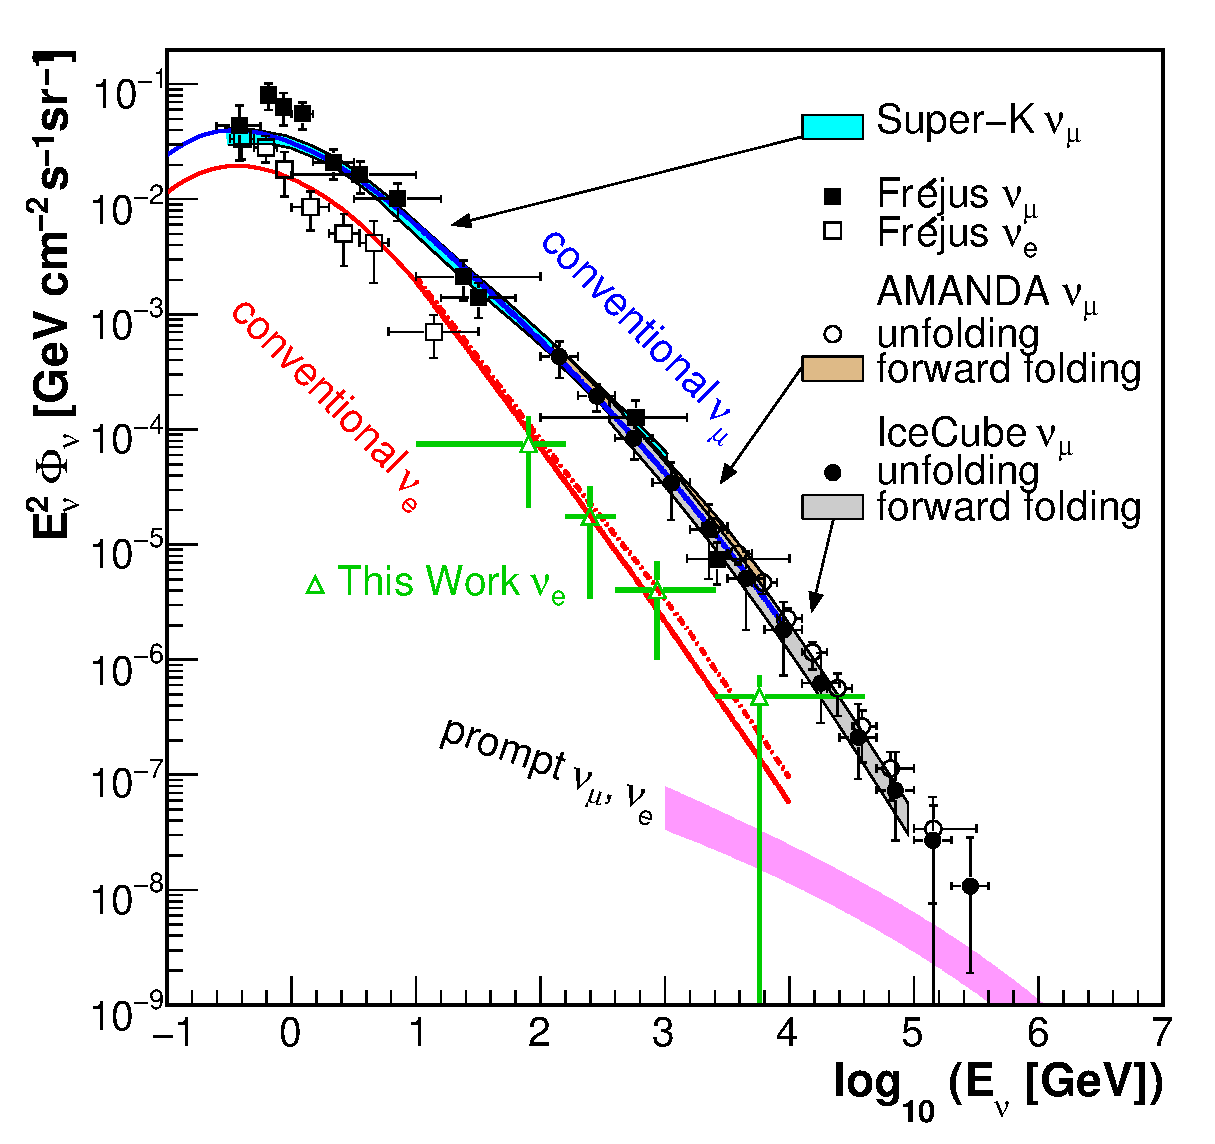
\includegraphics[height=7cm]{AtmFlux}}
  \caption{Spectra of the cosmic radiation at Earth and the resulting
    atmospheric neutrino spectrum.}
\label{fig:cosmic_rays_atm_nus}
\end{figure}

The origin of the cosmic radiation is not fully established yet. However it is
commonly assumed that the particles are accelerated in non-thermal processes,
usually moving shock fronts, that develop in extreme astrophysical environments.
This mechanism is known as Fermi acceleration \cite{FermiAcc}. 
Candidates for the acceleration sites are both galactic sources, such as
supernova remnants, as well as extragalactic ones like gamma ray bursts or
active galaxies. Due to their small size and rather low energy density, galactic
sources are believed to dominate the low-energy part of the spectrum in the GeV
to TeV regime, while the extragalactic contribution takes over at the knee
region.

When such a high energy particle hits the Earth's atmosphere, it interacts with
a nucleus in the air (usually nitrogen or oxygen) in a so-called deep-inelastic
scattering process. Since the energy of the incoming particle is far beyond all
binding energies in the nucleus, it is completely disrupted. From the fragments
of the nucleus that are still highly energetic, a shower of secondary particles
develops, that then travels down to Earth.

Main components of these particle showers are muons and pions. Both particles
are relatively short-lived\footnote{$\tau_\mu = 2.2 \times 10^{-6}$\,s,
$\tau_K = 1.2 \times 10^{-8}$\,s, and $\tau_\pi = 2.6 \times 10^{-8}$\,s
\cite{PDG}} and produce neutrinos in their decay:
\begin{eqnarray}
 \pi^\pm &\to\ & \mu^\pm + \numu(\numubar)  \label{eqn:pi_decay} \\
 K^\pm   &\to\ & \mu^\pm + \numu(\numubar) \\
 \mu^\pm &\to\ & e^\pm + \nue(\nuebar) + \numubar(\numu)
\end{eqnarray}
As one can see from the above equations, these so-called conventional
atmospheric neutrinos coming mostly from pion and kaon decays have a flavour
ratio of $\overset{(-)}{\numu}:\overset{(-)}{\nue} = 2:1$.

Their energy spectrum is linked to the primary spectrum of cosmic rays since the
secondary pions and muons follow the primary energy distribution directly. Thus
being highly relativistic, their lifetime is Lorentz boosted by a factor $\gamma
\propto E$. So the higher the particle's energy, the higher is 
its probability \emph{not} to decay into neutrinos in-flight but reach the
Earth's surface and interact there, producing another shower of much less
energetic particles. Therefore, the spectrum of conventional atmospheric
neutrinos is suppressed roughly by a factor of $1/E$ with respect to the primary
cosmic ray distribution.

For a more precise calculation, details of high-energy proton interactions and
the geomagnetic field have to be taken into account \cite{Honda2007, Bartol}. As
shown in Fig.~\ref{fig:cosmic_rays_atm_nus}, these predictions show good
agreement with measurements.

Another predicted, but not yet observed component of the atmospheric neutrino
flux are the so-called prompt neutrinos. They originate from charmed mesons 
that are rarely produced in cosmic ray induced air showers as well. Since these
are so short-lived that they always decay in-flight (``promptly'') despite of
their relativistic boost, their energy spectrum is the same as the primary one
and thus harder than the conventional component, but with a much smaller
normalisation.

% \subsection{Supernova Neutrinos}
% TODO: mention them?

\subsection{Astrophysical Neutrinos}

The highest energy neutrinos are the so-called astrophysical ones. They are  
assumed to be produced at similar sites as the cosmic radiation, i.\,e.\ in 
highly energetic shock fronts. There, $\Delta$ resonances are generated in the 
collision of protons and high-energy photons, producing pions in their decay:
\begin{equation}
 p + \gamma \to \Delta^+ \to n + \pi^+\ (p + \pi^0)
\end{equation}
The pions then decay further into neutrinos as shown in (\ref{eqn:pi_decay}).

Since astrophysical neutrinos are produced in the same processes as cosmic 
rays, their fluxes are linked. The flux of cosmic rays has been measured in 
quite some detail over the recent decades \cite{CosmRaySpec}, hence an upper 
limit for the flux of astrophysical neutrinos can be derived that is 
independent of any model assumptions about the production sites \cite{WB_bound}.

The first high energy astrophysical neutrino events have been recorded only
recently by the IceCube neutrino telescope \cite{HESE, HESE_3yr}, making them
the  highest energy neutrinos ever observed. Although event statistics are
still low, the flux seems to be very close to the predicted upper bound, meaning
that  the neutrino production efficiency is close to maximal. The spectral shape
of the flux is compatible with a power law with an index of --2 and an
exponential cut-off around a few PeV as well as a steeper
power law with index --2.3 \cite{Lars_globalfit}.

\section{Detection of Neutrinos}
\label{sec:NuDetection}

As already mentioned, neutrinos only interact with other particles in weak
processes where the total cross-sections are typically very low. Thus high
fluxes or large target volumes (or both) are needed to detect a sufficient
number of neutrinos.

And even if these requirements are fulfilled, in most cases the neutrino signal
has to be distinguished from a background of dominant processes, whose rate
can be several orders of magnitude higher than the neutrino event rate.
Depending on the targeted energy range, the most common background processes are
inherent radioactivity of the surroundings and the detector itself at MeV
energies, and muons created in cosmic ray induced air showers which can
penetrate even strong shielding.

\subsection{Neutrino cross-sections}
\label{sec:Xsecs}

The calculation and experimental testing of neutrino cross-sections has been a
field of extensive research over the past decades. On the experimental side,
the challenge is the smallness of the cross-sections. The key point on the
theoretical side is the calculation of the matrix elements associated with the
interaction of interest.

\begin{figure}[b]
 \vspace{\baselineskip}
 \centering
 \begin{fmffile}{nue_e_CC}
 \parbox{50mm}{
  \begin{fmfgraph*}(40,30) \fmfpen{thin}
    \fmfstraight
    \fmfleft{i00,i0,i2,i3,i41,i42,i5,i51,i6,i1}
    \fmfright{o00,o0,o2,o3,o41,o42,o5,o51,o6,o1}
    \fmf{fermion}{i0,v0,o0}
    \fmflabel{$e^-$}{i0}
    \fmflabel{$\nue$}{o0}
    \fmf{fermion}{i1,v1,o1}
    \fmflabel{$\nu_f$}{i1}
    \fmflabel{$f^-$}{o1}
    \fmf{dashes,lab=$W$,l.side=left,tension=1.}{v0,v1}
  \end{fmfgraph*}
  } + \qquad \quad
 \parbox{50mm}{
  \begin{fmfgraph*}(40,30) \fmfpen{thin}
    \fmfstraight
    \fmfleft{i00,i0,i2,i3,i41,i42,i5,i51,i6,i1}
    \fmfright{o00,o0,o2,o3,o41,o42,o5,o51,o6,o1}
    \fmf{fermion}{i0,v0,o0}
    \fmflabel{$e^-$}{i0}
    \fmflabel{$e^-$}{o0}
    \fmf{fermion}{i1,v1,o1}
    \fmflabel{$\nue$}{i1}
    \fmflabel{$\nue$}{o1}
    \fmf{dashes,lab=$Z^0$,l.side=left,tension=1.}{v0,v1}
  \end{fmfgraph*}
 }
 \end{fmffile}
 \write18{mpost nue_e_CC}
 \caption{Feynman diagrams for the charged (left) and neutral (right) current
  contributions of $\nu_f\,e^- \to \nue\,f^-$ scattering.}
\label{fig:nue_e_CC}
\end{figure}

As an introductory example, we will look at neutrinos scattering off a free
lepton. The cross-section is \cite{NuXsec_review}
\begin{equation}
 \frac{d\sigma}{dq^2} = \frac{1}{16\pi} \frac{|\mathcal{M}^2|}{(s-m_e^2)^2}\ ,
\end{equation}
with $s$ and $q^2$ being the centre-of-mass energy and the four-momentum
transfer, respectively, assuming very small neutrino mass. In this case,
calculating the matrix element $|\mathcal{M}^2|$ is rather straightforward,
since only weak interactions between fundamental particles have to be
considered. The scattering process itself is the sum of a charged-current
($W^\pm$ exchange, CC) and a neutral current ($Z^0$ exchange, NC) contribution,
as shown in Fig.~\ref{fig:nue_e_CC}.

\begin{figure}[t!]
 \centering
 \includegraphics[width=0.7\textwidth]{NuXsec_fullrange}
\caption{Electroweak cross-section for $\nue e^- \to \nue e^-$ scattering
  on free electrons as a function of neutrino energy. Various neutrino sources
  are also shown at their respective energy scales. \cite{NuXsec_review}}
 \label{fig:nue_e_xsec}
\end{figure} 

After converting the momentum transfer to the energy fraction $y$ carried by
the outgoing lepton, $\frac{dq^2}{dy} = 2m_e E_\nu$, the charged current
cross-section for scattering off an electron is given by \cite{NuXsec_review}
\begin{equation}
 \frac{d\sigma}{dq^2}\bigg\rvert_\mathrm{CC} = \frac{2m_e G_F^2 E_\nu}{\pi}
  \left(1 - \frac{m_f^2 - m_e^2}{2m_e E_\nu}\right)\ ,
 \label{eqn:nue_e_xsec}
\end{equation}
where $E_\nu$ is the incoming neutrino energy, and $m_e$ and $m_f$ are the
masses of the electron and the outgoing fermion. The corresponding total
cross-section for $\nue e^- \to \nue e^-$ scattering is shown in
Fig.~\ref{fig:nue_e_xsec}. In case that $m_f$ can be neglected compared to the
neutrino energy, the above can be integrated to give a simple expression for
the total cross-section:
\begin{equation}
 \sigma \simeq \frac{2m_e G_F^2 E_\nu}{\pi} = \frac{G_F^2 s}{\pi}
\end{equation}
In Fig.~\ref{fig:nue_e_xsec}, this corresponds to the regime above about
$10^7$\,eV, well above the electron mass. The sharp peak at $\sim 10^{16}$\,eV
is the so-called Glashow resonance, at which the centre-of-mass energy is
comparable to the $W$ boson mass, enabling resonant production of real $W^-$
bosons and hence causing a strong enhancement of the cross-section.

% TODO: also write down nubar  and NC cross-section?

When looking at other scattering processes, the principles of deriving the
cross-section remain the same. However the kinematic part is subject to change,
mostly due to different angular momentum states, and of course the matrix
elements depend strongly on the respective target. For non-fundamental targets,
form factors describing the internal charge distribution have to be taken
into account as well.

In general, the cross-section for hadronic interactions are much larger than the
leptonic ones (e.\,g.\ neutrino-electron scatting as discussed above) due to the
larger target masses. This means that for conventional targets consisting of
atoms with a nucleus and an electron hull, a neutrino is much more likely to
interact with the nuclei than with the shell electrons.

\subsection{Neutrino interactions with hadrons at the GeV scale}
\label{sec:XsecsGeV}

\begin{figure}
\centering
  \subfloat
    {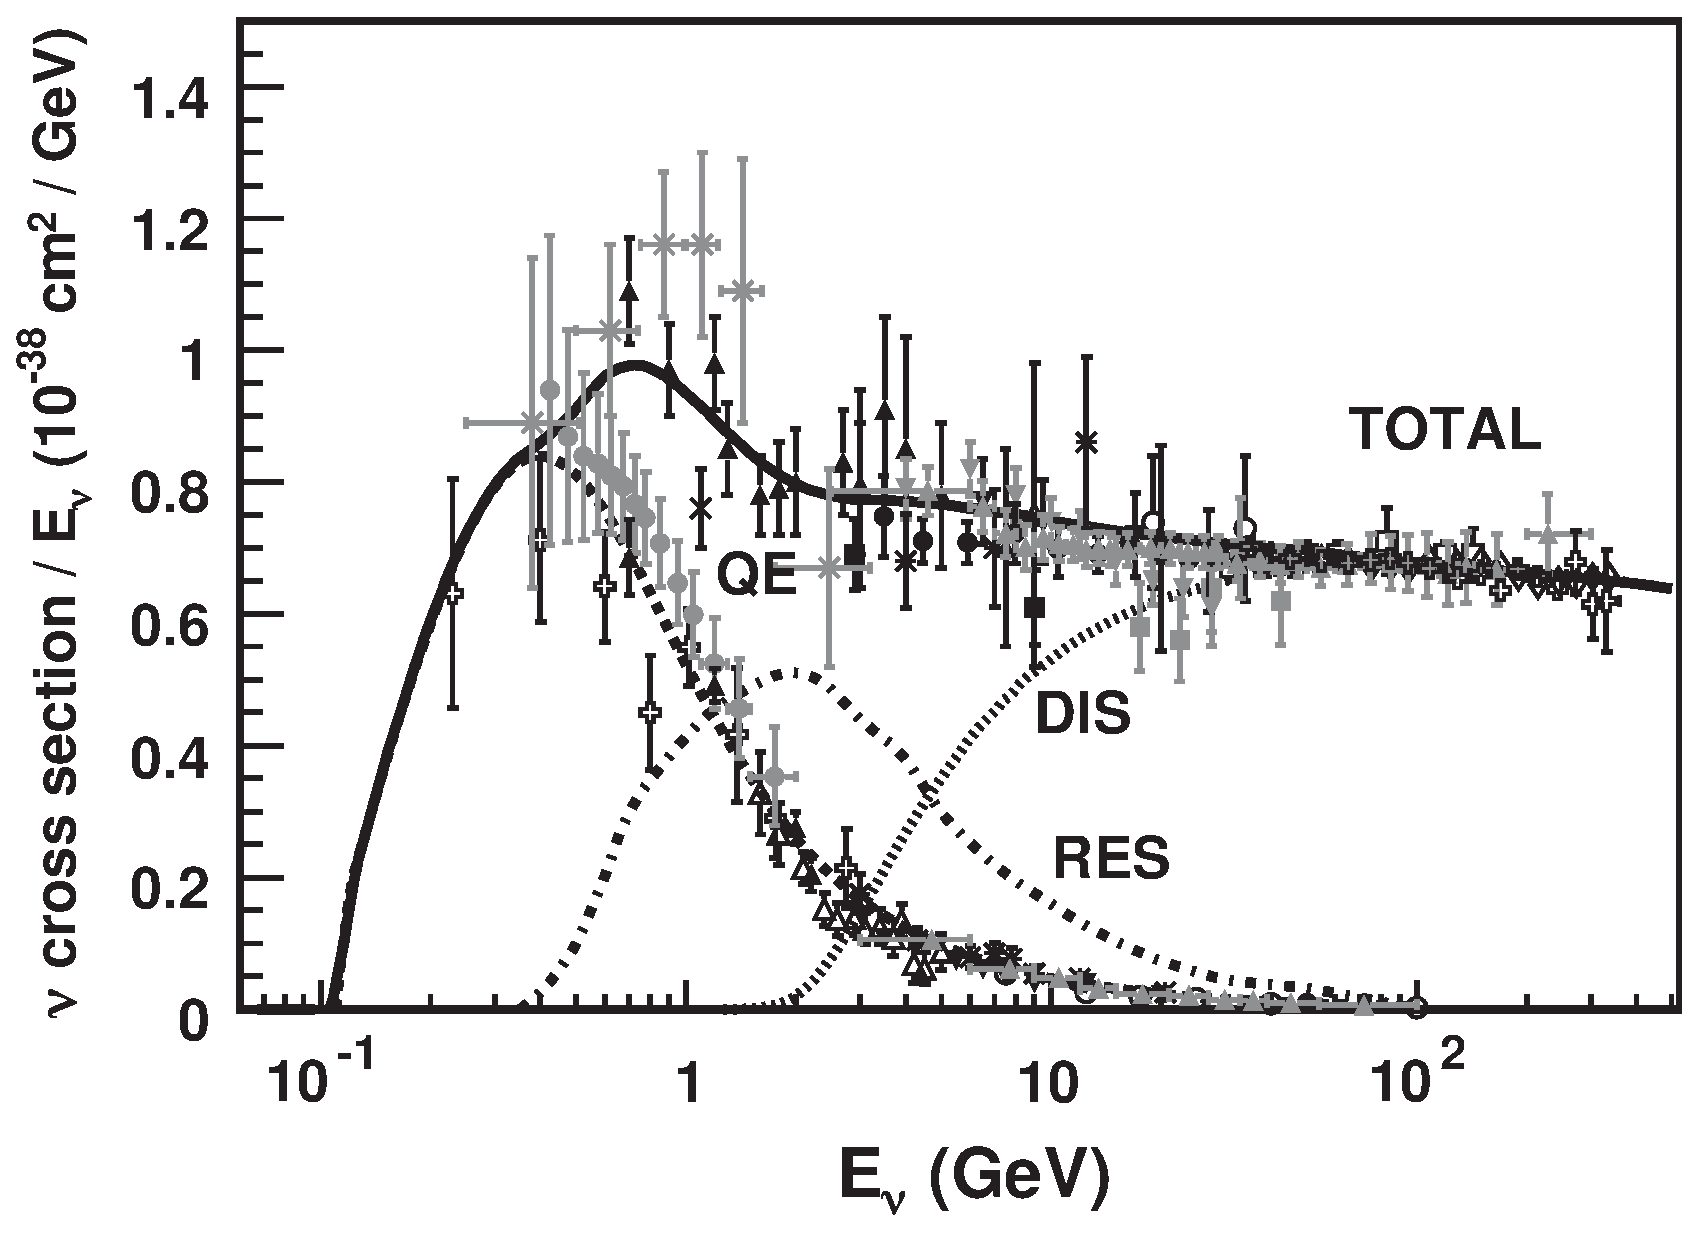
\includegraphics[width=7cm]{nu_N_xsec}}\qquad
  \subfloat
    {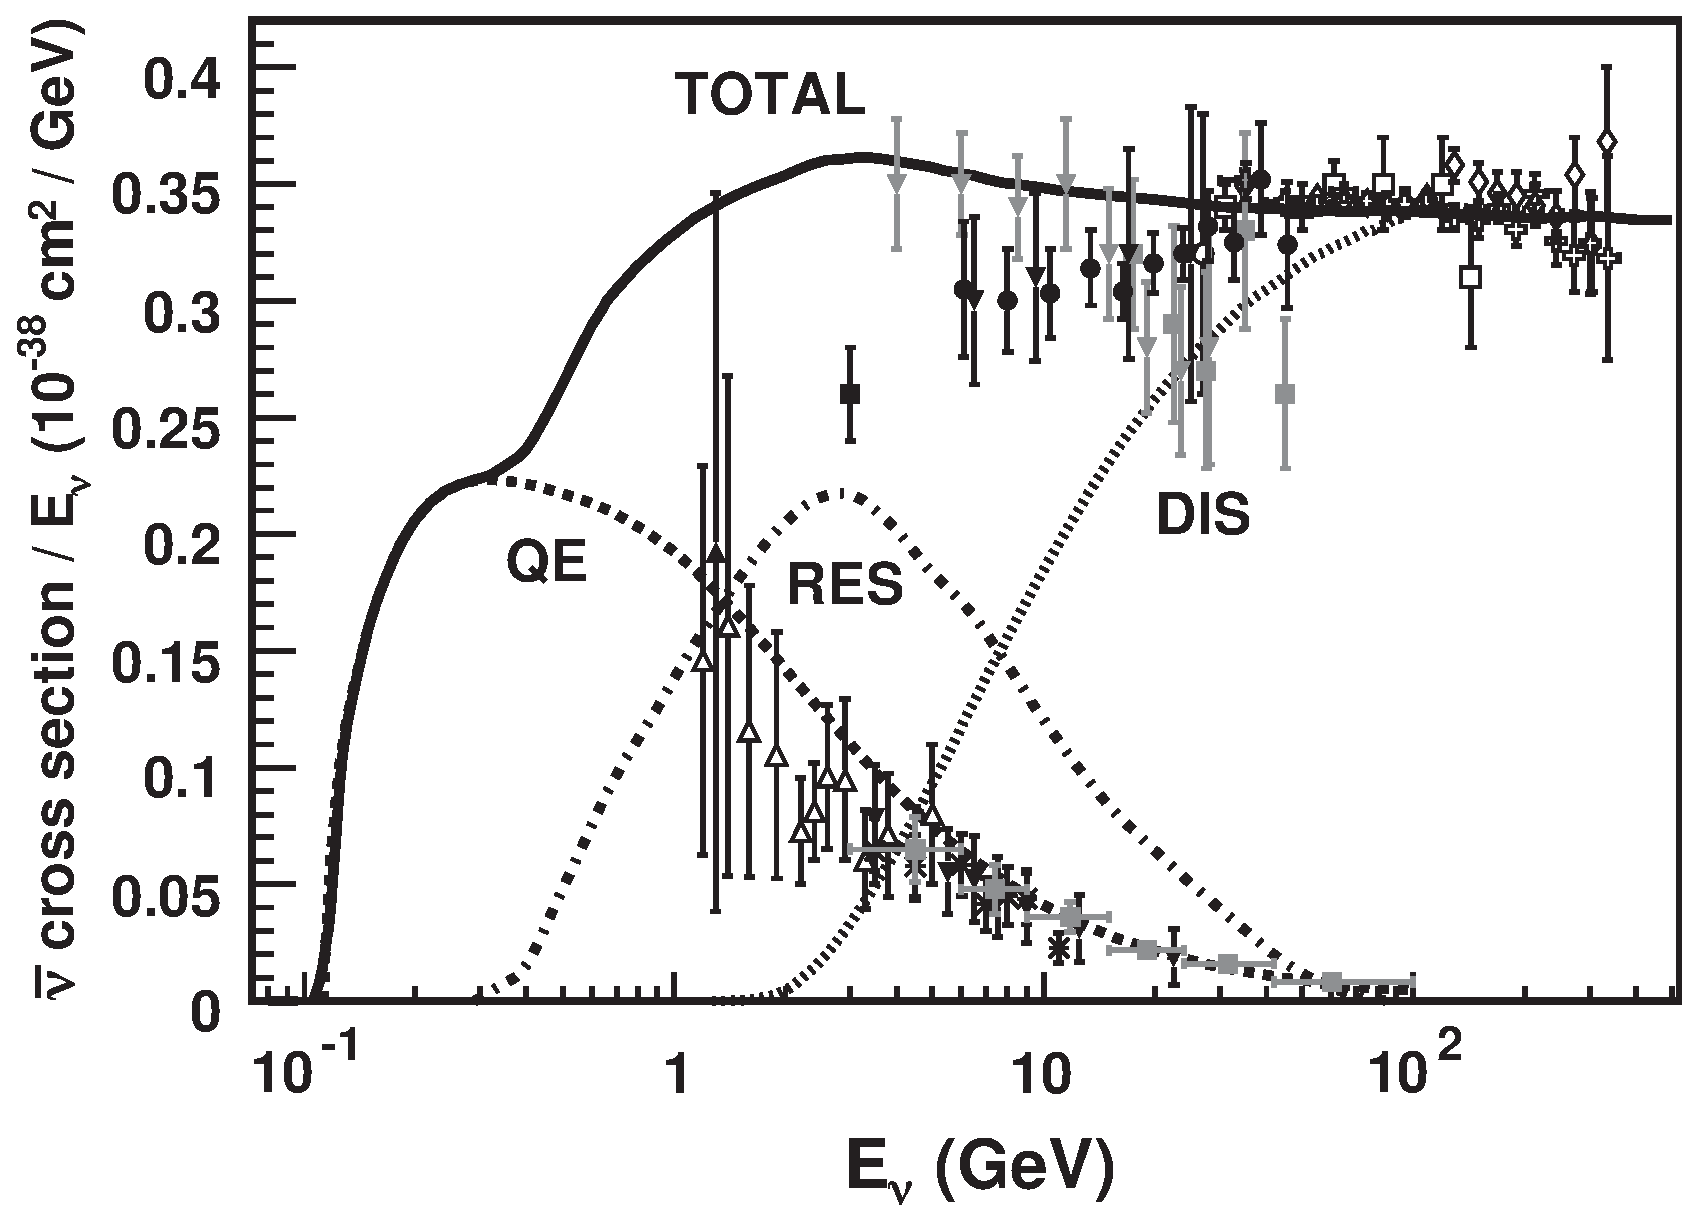
\includegraphics[width=7cm]{nubar_N_xsec}}
  \caption{Total CC cross-section for neutrino (left) and antineutrino
   (right) cross-section for an isoscalar nucleon, $N=(p+n)/2$, divided by the
   neutrino energy and plotted as a function of energy. Shown are data from
   various experiments and predictions for the quasi-elastic (QE), resonance
   (RES), and deep inelastic (DIS) contributions \cite{NuXsec_review}.}
\label{fig:NuXsec_GeV}
\end{figure}

For the scope of this thesis, the most interesting energy regime is the low GeV
scale, especially the range of $1 - 50$\,GeV. Here the cross-section for
neutrino interactions with nuclei is quite complex to describe, as several
distinct processes (shown in Fig.~\ref{fig:NuXsec_GeV}) have to be considered
for the scattering:
\begin{description}
 \item[Quasi-elastic scattering:] At rather low energies, the neutrino
    scatters off an entire nucleon, removing it (possibly together with other
    nucleons) from the nucleus. The free proton(s) or neutron(s) will then
    propagate through the surrounding medium until they have dissipated all
    their energy. These interactions range out quickly above about 10\,GeV.
 \item[Resonance production:] At the range of about $1-3$\,GeV, the
    dominant process is the excitation of short-lived baryonic resonances
    (such as $\Delta^+$ or $N^*$) in the target nucleon. These resonances then
    decay to various final states producing nucleons and $\pi$ mesons.
 \item[Deep inelastic scattering:] Above about 10\,GeV, the scattering
    neutrino has sufficient energy to resolve the quark structure of the
    nucleons. Then it scatters on a quark constituent rather than the whole
    nucleon. Thereby the nucleon gets disrupted and an hadronic shower
    consisting of a variety of mesons forms from its remains.
\end{description}

Common to all these processes is that they have both a CC and a NC
contribution---similar to the scattering off electrons shown in
Fig.~\ref{fig:nue_e_CC}, only that the target is either a whole (for
quasi-elastic and resonant processes) or a quark inside a nucleon (deep
inelastic scattering).

\begin{figure}
 \centering
 \begin{fmffile}{nux_NC}
 \begin{fmfgraph*}(50,30) \fmfpen{thin}
 \fmfstraight
  \fmfleftn{i}{8}
  \fmfrightn{o}{8}
  \fmf{heavy}{i2,v1}
  \fmfv{decor.shape=circle,decor.filled=shaded}{v1}
  \fmf{vanilla}{v1,o2}
  \fmflabel{nucleus}{i2}
  \fmflabel{hadronic\ shower}{o2}
  \fmf{fermion}{i8,v2,o8}
  \fmflabel{$\nu$}{i8}
  \fmflabel{$\nu'$}{o8}
  \fmf{dashes,lab=$Z^0$,l.side=left,tension=1.5}{v1,v2}
  \fmffreeze
  \fmf{vanilla}{v1,o1}
  \fmf{vanilla}{v1,o3}
 \end{fmfgraph*}
 \end{fmffile}
 \write18{mpost nux_NC}
\caption{Neutral current interaction between a neutrino and a nucleus.}
\label{fig:nux_NC}
\end{figure}

This means that four different classes of events can be observed. The first are
neutral current interactions of any neutrino flavour, as shown in
Fig.~\ref{fig:nux_NC}. In this case, the final state consists of the scattered
neutrino $\nu'$ and a hadronic shower or cascade consisting of a variety of
mesons, fermions, and photons developing from the fragments of the stricken
nucleus.

The details of the development of such a hadronic shower are not fully
understood and have to be modelled in MonteCarlo based simulations. However,
since the involved particles are mostly short-lived and strongly interacting,
the typical size is on the order of one meter or below. 

The outgoing neutrino on the other hand is virtually impossible to detect,
meaning that the fraction of the total interaction energy that is carried by
this neutrino remains invisible. In beam experiments, in which the energy of the
incoming particles is known, this is commonly referred to as ``missing energy''.

\begin{figure}
\centering
  \subfloat[\label{fig:nue_CC}]
    {
     \begin{fmffile}{nue_CC}
      \begin{fmfgraph*}(30,20) \fmfpen{thin}
      \fmfstraight
        \fmfleftn{i}{8}
        \fmfrightn{o}{8}
        \fmf{heavy}{i2,v1}
        \fmfv{decor.shape=circle,decor.filled=shaded}{v1}
        \fmf{vanilla}{v1,o2}
        \fmf{dashes,lab=$W$,l.side=left}{v1,v2}
        \fmf{fermion}{i7,v2}
        \fmflabel{\nue}{i7}
        \fmf{phantom}{v2,o7}
        \fmffreeze
        \fmf{fermion,lab=$e$,l.side=left,tension=2}{v2,v3}
        \fmf{vanilla}{v3,o7}
        \fmflabel{EM\ shower}{o6}
        \fmf{vanilla}{v1,o1}
        \fmf{vanilla}{v1,o3}
        \fmf{vanilla}{v3,o6}
        \fmf{vanilla}{v3,o8}
      \end{fmfgraph*}
     \end{fmffile}
     \write18{mpost nue_CC}
    }\qquad\qquad
  \subfloat[\label{fig:numu_CC}]
    {
     \begin{fmffile}{numu_CC}
      \begin{fmfgraph*}(30,20) \fmfpen{thin}
      \fmfstraight
        \fmfleftn{i}{8}
        \fmfrightn{o}{8}
        \fmf{heavy}{i2,v1}
        \fmfv{decor.shape=circle,decor.filled=shaded}{v1}
        \fmf{vanilla}{v1,o2}
        \fmf{dashes,lab=$W$,l.side=left}{v1,v2}
        \fmf{fermion}{i7,v2,o7}
        \fmflabel{\numu}{i7}
        \fmflabel{$\mu$}{o7}
        \fmffreeze
        \fmf{vanilla}{v1,o1}
        \fmf{vanilla}{v1,o3}
      \end{fmfgraph*}
     \end{fmffile}
     \write18{mpost numu_CC}
    }\qquad\qquad
  \subfloat[\label{fig:nutau_CC}]
    {
     \begin{fmffile}{nutau_CC}
      \begin{fmfgraph*}(30,20) \fmfpen{thin}
      \fmfstraight
        \fmfleftn{i}{8}
        \fmfrightn{o}{10}
        \fmf{heavy}{i2,v1}
        \fmfv{decor.shape=circle,decor.filled=shaded}{v1}
        \fmf{vanilla}{v1,o2}
        \fmf{dashes,lab=$W$,l.side=left}{v1,v2}
        \fmf{fermion}{i7,v2}
        \fmflabel{\nutau}{i7}
        \fmf{phantom}{v2,o7}
        \fmffreeze
        \fmf{fermion,lab=$\tau$,l.side=left,tension=5}{v2,v3}
        \fmf{vanilla}{v3,o7}
        \fmflabel{hadr./EM\ shower}{o7}
        \fmf{vanilla}{v1,o1}
        \fmf{vanilla}{v1,o3}
        \fmf{vanilla}{v3,o6}
        \fmf{vanilla}{v3,o8}
        \fmf{fermion}{v3,o10}
        \fmflabel{\nutau}{o10}
      \end{fmfgraph*}
     \end{fmffile}
     \write18{mpost nutau_CC}
    }
  \caption{Charged current interactions between a \nue (a), \numu (b), and
           \nutau (c) and a nucleus.}
\label{fig:nu_CC}
\end{figure}

In charged current interactions, the neutrino scatters off a nucleus by
exchanging a $W$ boson. From the fragmented nucleus, a hadronic shower develops
similarly to the neutral current case. The outgoing lepton however is now a
charged one, the flavour corresponding to the incoming neutrino's flavour. This
charged lepton now dominates the event signature:

\begin{description}
 \item[Electron:] In dense matter, a GeV electron will trigger an
  electromagnetic shower by radiating high-energy photons (bremsstrahlung),
  which in turn will create electron-positron pairs. The typical scale length
  $X_0$ of such a shower is given by
  \begin{equation}
   \frac{1}{X_0} = 4\alpha r_e^2 \frac{N_A}{A}
                    \left\{ Z^2 \left[L_\mathrm{rad} - f(Z) \right]
                    + Z\,L_\mathrm{rad}'\right\} \quad,
   \label{eqn:rad_length}
  \end{equation}
  where $\alpha$ is the fine structure constant, $r_e$ the classical electron
  radius, and $N_A$ Avogadro's number. $A$ and $Z$ are atomic mass and charge
  of the medium, and $L_\mathrm{rad}$, $L_\mathrm{rad}'$, and $f(Z)$
  semi-empirical parameters that have been tabulated \cite{PDG, bremsstrahlung}.
  For water, the scale length is $X_\mathrm{0,\,H_2O} =
  24.33\,\mathrm{g/cm}^2$, meaning that the typical size of such a shower is
  about one metre, as water has a density of $\varrho_\mathrm{H_2O} =
  1$\,g/cm$^3$.
 \item[Muon:] In contrast to the much lighter electron, a muon of a few GeV is
  a so-called minimum ionising particle. This means it is in the minimum region
  of the Bethe-Bloch formula for the energy loss of a charged particle in
  matter:
  \begin{equation}
   \left\langle -\frac{dE}{dx}\right\rangle = Kz^2\frac{Z}{A}\frac{1}{\beta^2}
      \left[ \frac{1}{2}\ln\frac{2m_ec^2\beta^2\gamma^2 W_\mathrm{max}}{I^2}
             - \beta^2 - \frac{\delta(\beta\gamma)}{2} \right] \quad.
   \label{eqn:bethe-bloch}
  \end{equation}
  Here, $K = 4\pi N_A r_e^2 m_ec^2$, $z=1$ is the electrical charge of the
  muon, $I$ the mean excitation potential of the material, $\delta(\beta\gamma)$
  a density effect correction, and $W_\mathrm{max}$  the maximum energy transfer
  in a single collision between the muon and an  electron in the medium.
  $\beta = v/c$ and $\gamma$ are the Lorentz variables \cite{PDG}.

  This expression has a wide minimum in the range $\beta\gamma\approx 1 - 100$, 
  corresponding to a muon momentum in the low GeV/$c$ regime. Here,
  (\ref{eqn:bethe-bloch}) evaluates to $\langle dE/dx\rangle \approx
  2$\,MeV/(g/cm$^2$), hence for a medium with a density of 1\,g/cm$^3$ a muon
  has a range of approximately 5\,m/GeV before it has deposited all its energy
  and decays at rest.
 \item[Tau:] In principle, a tau lepton is a minimum ionising particle as well.
  But with a lifetime of only $2.9\times10^{-13}$\,s and a mass of 1.78\,GeV, at
  GeV energies it can travel at most a few hundred microns before it decays. In
  its decay, a \nutau has to be created again, whose energy has to be considered
  ``missing'' as well. The remaining decay products form an electromagnetic or
  hadronic shower, depending on their nature.
\end{description}

In a large detector with detection units spaced widely on a scale of several 
meters, like the PINGU neutrino telescope described in Sec.~\ref{sec:PINGU}, the
four event classes discussed above can only be categorized into two channels: 
tracks and cascades. 
\begin{description}
 \item[Tracks] correspond to \numu CC events. A muon track of several meters 
  length is pointing away from the hadronic shower at the event vertex. In 
  principle, this allows for a good directional reconstruction of the event. 
  For the energy reconstruction on the other hand there is the disadvantage 
  that the outgoing muon might not be fully contained in the detector, then 
  only a fraction of its total energy can be recorded.
 \item[Cascades] encompass all other types of events. A hadronic shower is 
  always present, and another shower of electromagnetic or hadronic nature 
  overlays it, if a CC interaction has occurred. The displacement of the second 
  shower (if it exists) is far smaller than a millimetre and hence not 
  resolvable. Also the showers themselves have to be considered point-like, but 
  have some directionality since the momentum of the incoming neutrino is 
  transferred to the final state. 
  
  The achievable directional resolution is still worse than for tracks since 
  the events lack a long lever arm in form of an extended muon trajectory. Yet 
  the energy resolution should be better at least for \nue CC events, since the 
  event is always fully contained in the detector. For NC and \nutau CC events 
  the energy of the outgoing neutrino in the final state is invisible, causing 
  a reconstruction bias towards low energy.
\end{description}


\subsection{Cherenkov Effect}
\label{sec:Cherenkov}

As discussed above, high fluxes and/or large target volumes are required for 
the detection of neutrino interactions. Since the atmospheric flux is rather 
low compared to focused, high-intensity artificial beams, there is no way 
around building a megaton scale detector when searching for atmospheric 
neutrinos. Obviously, a ``conventional'' detector for subatomic 
particles\footnote{made up from e.\,g.\ wire chambers, solid state 
scintillators, ...} is not feasible at these dimensions.

The common choice for measuring natural (i.\,e.\ low) neutrino fluxes above 
MeV energies are water-based Cherenkov detectors. A large volume of water or 
ice serves as both target and detector: The neutrinos interact with the protons 
and neutrons in the water molecules, creating relativistic charged particles as
described in the previous section. Then the charged particles emit light via the
Cherenkov effect, which propagates in the transparent medium and can finally be
detected (usually using photomultiplier tubes) to reconstruct the underlying
neutrino event.

\begin{figure}
  \centering
  \includegraphics[width=0.4\textwidth]{Cherenkov}
  \caption{Illustration of the Cherenkov effect (schematic). Photons are
    emitted perpendicular to the surface of the Cherenkov cone at the angle
    \thet{\mathrm{C}}, as indicated by the arrow. Graphics taken from
    \cite{Jackson}.}
\label{fig:Cherenkov}
\end{figure}

Whenever a charged particle moves through a dielectric medium, it shortly 
polarises the atoms along its path, which in turn emit electromagnetic waves. 
Usually waves from neighbouring cancel, such that no net effect is observable. 
If, however, the velocity of the charged particle is higher than the local 
phase velocity of light given by the index of refraction,
\begin{equation}
 v > c_{\mathrm{medium}} = c/n \quad,
\end{equation}
the wave fronts interfere constructively to form a shock front of conical 
shape, similar to the Mach cone in supersonic motion (see 
Fig.~\ref{fig:Cherenkov}). Photons are emitted almost\footnote{As group and 
phase velocity differ, the angle is not quite 90\textdegree.} rectangular to 
the shock front.

The opening angle of the Cherenkov cone is given by the relation
\begin{equation}
  \cos \vartheta_{\mathrm{Ch}} = 
      \frac{c_{\mathrm{medium}}}{v} = \frac{1}{\beta n} \quad.
\end{equation}
It depends on the particle's velocity and hence its energy. Usually, the 
constituents of the particle showers are relativistic, so $\beta \simeq 1$ and 
hence 
\begin{equation}
  \vartheta_{\mathrm{Ch}} \simeq \arccos \frac{1}{n_{\mathrm{ice}}} 
      \simeq \mathrm{41^{\circ}}
  \label{eqn:ChkovAngle}
\end{equation}
for ice with $n_{\mathrm{ice}} \simeq 1.32$ \cite{PriceWoschnagg}.

The energy loss due to Cherenkov radiation is described by the Frank-Tamm 
formula that can be found in \cite{Jackson}:
\begin{equation}
  \frac{dE}{dx} = \frac{(Z e)^2}{c^2} \int_{n(\omega)>1/\beta^2} \omega 
    \left( 1 - \frac{1}{(\beta n(\omega))^2} \right) d\omega \quad.
\end{equation}
This integral does not diverge as the refractive index drops below 1 in the 
ultraviolet region.

Its contribution to the total energy dissipation of the particle\footnote{Which 
is described by the Bethe-Bloch formula (\ref{eqn:bethe-bloch}).} is marginal, 
but from this the rate of photon production can be inferred. Expressed as an 
energy spectrum, the number of photons generated per track length is
\cite{PDG}
\begin{equation}
  \frac{d^2 N_{\gamma}}{dx\,dE} 
    = \frac{\alpha Z^2}{\hbar c} \sin^2 \vartheta_{\mathrm{Ch}}
    = \frac{\alpha Z^2}{\hbar c} \left(1-\frac{1}{(\beta n(E))^2}\right) \quad,
\end{equation}
where for simplicity the refractive index was treated as constant. Evaluating 
the constants, one finds for particles of unit charge ($Z^2 = 1$) in polar ice:
\begin{equation}
  \frac{d^2 N_{\gamma}}{dx\,dE} 
    \approx 370\,\sin^2\vartheta_{\mathrm{Ch}}\,\mathrm{eV}^{-1}\mathrm{cm}^{-1}
    \approx 175 \,\mathrm{eV}^{-1}\mathrm{cm}^{-1} \quad.
\end{equation}
One also often finds a version of this formula giving a wavelength spectrum 
\cite{PDG}:
\begin{equation}
  \frac{d^2 N_{\gamma}}{dx\,d\lambda} = \frac{2\pi\alpha Z^2}{\lambda^2}
    \left(1-\frac{1}{(\beta n(\lambda))^2}\right) \quad.
  \label{eqn:FrankTammWvl}
\end{equation}
Here the $1/\lambda^2$ dependency of the spectrum becomes evident\footnote{This 
is the reason for the bright blue colour in which Cherenkov light appears to 
the human eye.}. When using this wavelength dependent equation, one has to bear 
in mind that $\lambda$ always means the \emph{vacuum} wavelength and not the 
wavelength in the medium that differs from that in the vacuum by a factor of 
$n$.

As mentioned above, the energy dependent expression can be treated as constant 
with good accuracy. Then the integration over a certain energy interval becomes 
trivial and one can easily estimate the number of Cherenkov photons for a
certain particle. Again using the values for polar ice, the calculation yields a 
number of
\begin{equation}
  \frac{dN_{\gamma}}{dx} \approx 325 \,\mathrm{cm}^{-1}
  \label{eqn:Chkov_Nphot_per_track_length}
\end{equation}
photons in the visible range between 300\,nm and 600\,nm of vacuum wavelength. 

%==============================================================================
\section{Neutrino Oscillations}
\label{sec:osc}
%==============================================================================

The Standard Model of Particle Physics, as described in the previous section,
has been one of the most successful theories in the history of physics. It is,
however, not fundamental in the sense that it can explain all physical
phenomena alone. Its shortcomings are e.\,g.\ the missing inclusion of the
fourth fundamental force, gravity, and an explanation of the fundamental
asymmetry between bosons and fermions.
There are theoretical extensions to the Standard Model addressing these
questions, such as quantum gravity \cite{QuantumGravity} and supersymmetry
\cite{SUSY}, but all of them lack experimental evidence so far.

Yet there is one effect of so-called ``Physics beyond the Standard Model'' that
has been well established experimentally during the past years: neutrino
oscillations. As already mentioned in Sec.~\ref{sec:NusInSM}, this term refers
to neutrinos changing their flavour when travelling over macroscopic distances,
which can be explained by finite neutrino masses, while in the Standard Model
they have zero mass. The theory behind this process will be described in the
following.

\subsection{Vacuum Oscillations}
\label{sec:VacOsc}

There are two bases of eigenstates to which a neutrino can be decomposed: the
flavour and the mass base. The flavour eigenstates are \ket{\nue}, \ket{\numu},
and \ket{\nutau}, which will be summarised as \ket{\nu_\alpha}. These are the
eigenstates of the weak interaction, hence neutrinos are always produced as a
pure flavour eigenstate and have to be projected back onto these eigenstates
whenever they interact.

On the other hand there are the three mass eigenstates \ket{\nu_1}, \ket{nu_2},
and \ket{\nu_3}, summarised as \ket{\nu_i}, corresponding to the three neutrino
masses $m_i$. The absolute values of these masses are yet unknown, but since
neutrino oscillations have been observed, at least two of them have to be
different from zero. The mass eigenstates have to be considered when describing
the propagation of a neutrino in vacuum since the corresponding Hamiltonian
\begin{equation}
 \hat{H} = -\frac{\hbar^2}{2m}\nabla^2
\end{equation}
only depends on its mass.

Changes between the two bases are carried out via the so-called PMNS
matrix\footnote{After Bruno Pontecorvo, Ziro Maki, Masami Nagakawa, and Shoichi
Sakata}


\subsection{Neutrino Mass Hierarchy}
\label{sec:NMH}


\subsection{Oscillations in Matter}
\label{sec:MSW}


\subsection{Oscillation Experiments}
\label{sec:OscExp}

%==============================================================================
\chapter{Detector}
\label{sec:det}
%==============================================================================

In this chapter, a detailed description of the proposed PINGU neutrino
telescope and its predecessor IceCube will be given. We will start with
introducing the concept of ice or water based neutrino telescopes based on the
detection of Cherenkov radiation with IceCube/DeepCore as example, followed by
a characterisation of its upcoming PINGU upgrade.
Thereafter we will discuss how physics events will be selected and
reconstructed in an analysis targeting the determination of the neutrino mass
hierarchy, and finally how conceptually new hardware might improve the results.

%==============================================================================
\section{IceCube/DeepCore}
\label{sec:ICDC}
%==============================================================================

\subsection{Location}
\label{sec:IClocation}

As already mentioned (Sec.~\ref{sec:NuDetection}), the natural choice for
observing the low natural fluxes of high energy neutrinos are water-based
Cherenkov detectors. Although the basic requirement---a sufficiently large
amount of water or ice---seems not very difficult to meet, there are additional
constraints that have to be addressed as well:

\begin{description}
 \item[Size:] Depending on the energy range one is interested in, the size of
  the detector has to be adjusted accordingly. Since the atmospheric flux
  decreases rapidly with increasing energy, one needs larger detectors to study
  higher fluxes. Roughly from the GeV scale upwards, the required dimensions are
  so big (several hundred metres) that artificial structures like the
  underground caverns of Kamiokande and Super-Kamiokande \cite{SuperKosc} are
  not feasible any more and one has to look for suitable natural locations.
 \item[Transparency:] Since the detection of neutrinos is based on recording
  Cherenkov radiation, i.\,e.\ photons in the optical and near UV regime,
  obviously the chosen medium has to be transparent for these photons. Here ice
  has an advantage over fluid water as it has very low absorption down to
  wavelengths of 300\,nm and below \cite{IceProps}, while the fluid starts to
  absorb significantly below 400\,nm \cite{WaterAbs}.
 \item[Purity:] Usually the experiments try to reconstruct the neutrino events
  as accurately as possible. Therefore it is desirable to record a large number
  of unscattered photons and hence a very clear environment\footnote{There might
  be, however, situations where scattering is desired, e.\,g.\ when only the
  neutrino energy is of interest, then strong scattering keeps the photons
  inside the detector for a longer time and hence increases the total number
  of detected photons, thereby improving the energy resolution}.
 \item[Shielding:] In high energy neutrino experiments, muons from atmospheric
  showers created by cosmic radiation (cf.\ Sec.~\ref{sec:AtmNus}) are a
  background process whose rate is several orders of magnitude higher than the
  neutrino signal. In order to suppress those muons, detectors have to be
  placed deep underground so that there is a shielding with several hundred
  meters thickness, comparable to the range of $\mathcal{O}
  (100\,\mathrm{GeV})$ muons.
\end{description}

\begin{figure}[htp]
 \centering
 \includegraphics[width=\textwidth]{Icepaper_figure22_scatt-abs-length}
 \caption{Effective scattering and absorption of light in the polar ice. Plot 
  taken from \cite{IceProps}.}
 \label{fig:ice_scatt_abs}
\end{figure}

Choosing an environment optimising all these factors, the IceCube neutrino 
observatory has been constructed in the deep glacial ice at the geographical 
South Pole in Antarctica. The Antarctic glacier with its thickness of $\approx 
2500$\,m is a pristine environment of substantial size. In contrast to natural 
resources like lakes or the deep sea, it inherently provides a solid holding 
structure for the instrumentation, is free of lifeforms that might disturb or 
even destroy the detector, and has a much lower content of radioactive $^{40}$K 
than sea water. Especially at depths more than $\approx 2000$\,m below the 
surface, age and high pressure have facilitated the hydratisation of enclosed 
air bubbles, leaving an extremely clear ice with scattering and absorption 
lengths of several tens of metres even in the UV range, see 
Fig.~\ref{fig:ice_scatt_abs}. Instrumenting only the deepest ice below 1500\,m 
guarantees a sufficient shielding of atmospheric muons. 

The nearby Amundsen-Scott South Pole Station operated by the United States 
Antarctic Program provides the infrastructure needed for such a large scale 
experiment. This incorporates the supply of electrical power for the detector 
itself and the computing farm processing the raw data, satellite communications 
for transmitting science data, general technical support as well as 
accommodations for the visiting scientists.

\subsection{Detector Geometry}
\label{sec:ICgeometry}

A total of 86 strings, each instrumented with 60 Digital Optical Modules (DOMs, 
see Sec.~\ref{sec:ICDOM}), have been installed during IceCube's deployment phase 
from 2005 until December 18, 2010. A hot water drill was used to melt holes of 
60\,cm diameter into the ice, reaching down to 2450\,m, shortly above the 
underlying bedrock. Then the strings were lowered into the holes still filled 
with water which then refroze and firmly encloses the strings.

Eighty of those strings form the hexagonal main array with an inter-string 
distance of 125\,m, while the remaining six are placed at additional positions 
near the centre of the array, forming a dense sub-array with a string spacing 
of only 72\,m, lowering the threshold energy for neutrino detection from 
$\approx 100$\,GeV to $\approx 20$\,GeV. A top view of the string layout is 
shown in Fig.~\ref{fig:string_layout}.

\begin{figure}[htp]
 \centering
 \includegraphics[width=\textwidth]{ic_dc_pingu_strings}
%  \includegraphics[width=0.7\textwidth]{pingu_V36_Zezel_40_s22_d3}
 \caption{Top view of the IceCube string layout, including the DeepCore and 
planned PINGU (geometry V36) sub-arrays.}
 \label{fig:string_layout}
\end{figure}

To the lowest 1000\,m of the main array strings, sixty DOMs each are attached, 
evenly spaced with a distance of 17\,m. In DeepCore, the vertical DOM spacing 
is only 7\,m below the dust layer found between 1950\,m and 2100\,m 
depth\footnote{The dust layer can be recognised easily in 
Fig.~\ref{fig:ice_scatt_abs} as the region of increased scattering and 
absorption.}, with a veto cap of ten DOMs with 10\,m spacing per DeepCore 
string above it \cite{I3Design,DCDesign}.


\subsection{Digital Optical Modules}
\label{sec:ICDOM}

\begin{figure}[htp]
 \centering
 \includegraphics[width=0.7\textwidth]{I3DOM_PDOM_cropped}
 \caption{Comparing an IceCube/DeepCore DOM to the PDOM used in PINGU. Graphics 
taken from \cite{PDOM_Aachen}.}
 \label{fig:DOM}
\end{figure}

The 5160 Digital Optical Modules are the basic detection units of IceCube. They 
are attached to the string and connected to the main string cable during 
deployment and work autonomously except for the low voltage power supply. This 
modular design has the convenience that if one DOM fails to work and cannot be 
fixed as it is frozen in the deep ice, the others are not affected.

As shown in Figure \ref{fig:DOM}, the DOM is housed by a borosilicate glass 
sphere of 13\verb+"+ diameter and 0.5\verb+"+ thickness to withstand the 
pressure arising from the refreezing water in the drill holes. This glass sphere 
also contributes to the noise rate of about 540\,Hz per DOM as it contains 
isotopes of the uranium and thorium decay chains. The content of natural 
$^{40}\mathrm{K}$, that undergoes beta decay where the emitted $\beta$ particle
generates Cherenkov light, has been reduced in the glass.

The main component of the DOM is a 10\verb+"+ photomultiplier tube (Hamamatsu 
R7081-02 \cite{PMTpaper,PMTdata}). In DeepCore, an improved version of this PMT 
with a 35\,\% higher quantum efficiency was used \cite{DCDesign}. The PMT is 
oriented downwards as the main focus of IceCube is on extraterrestrial neutrinos 
from the northern hemisphere that have travelled through the Earth and hence 
arrive at the South Pole from below. The coupling to the glass sphere is 
provided by an optical gel which also provides protection and fixation to the 
PMT, while a surrounding Mu-metal grid guarantees the shielding of external 
magnetic fields.

The upper half of the DOM is filled with an high voltage divider that locally 
transforms the 96\,V voltage that is provided by the string main cable into the 
high voltage of 1.3--1.5\,kV that is needed to fuse the PMT, thus making it 
independent from possible voltage fluctuations of the pole station's power 
supply. Around the HV divider, the circular flasher board and DOM mainboard are 
mounted. The flasher board is populated with LEDs that can be used to produce a 
standardised signal for calibration. On the mainboard the electronics are 
located that are needed to read out the PMT signal and digitise the recorded 
data in situ, after which they are sent to the surface.



%==============================================================================
\section{PINGU}
\label{sec:PINGU}
%==============================================================================

PINGU, the Precision IceCube Next Generation Upgrade, is planned as a further 
infill to the IceCube/DeepCore array, lowering the energy threshold to few GeV 
\cite{LoI}. The current baseline geometry, V36, consists of forty additional 
strings with 96 PINGU-DOMs (PDOMs, see below) each. In this layout, shown in
Figs.~\ref{fig:string_layout} and \ref{fig:string_layout}, the string spacing is
22\,m while the PDOMs are located the lowest 300\,m of IceCube with a vertical
distance of 3\,m. In this depth, the same as the main part of DeepCore, the ice
has the best optical properties.

\begin{figure}[htp]
 \centering
 \includegraphics[width=\textwidth]{ic_dc_pingu_sideview}
%  \includegraphics[width=0.7\textwidth]{pingu_V36_Zezel_40_s22_d3}
 \caption{Side view of the IceCube string layout, including the DeepCore and
  planned PINGU (geometry V36) sub-arrays. The approximate position of the dust
  layer is shown for reference.}
 \label{fig:string_layout_side}
\end{figure}

This detector geometry has been optimised to yield a maximum sensitivity for 
the neutrino mass hierarchy. It will be used for all studies described in 
Chapter~\ref{sec:ana} unless explicitly stated otherwise.

In terms of hardware and software infrastructure, many things can be adopted 
from IceCube, redesigning parts where a potential for improvement or 
simplification has been discovered. Several components of the electronics part
of the module, like the main board, the PMT base, and the high voltage supply,
have been redesigned or replaced by more recent versions. In particular the PMTs
will all be the high quantum efficiency models already installed in DeepCore.
A delay board has become obsolete with the more recent signal digitisers and
will not be part of the PINGU DOMs. Additional components, such as cameras to
monitor the freeze-in process, are in discussion.

Although the bulk of PDOMs are an improved version of the technology that has 
proven to work reliably, prototypes of novel optical modules will be deployed 
with PINGU as well. As those might be the baseline technology of future 
neutrino telescopes, they have to be tested under realistic conditions before 
they can be considered for large-scale use. Two options for these 
next-generation optical modules are described in Sec.~\ref{sec:Gen2DOM}, 
studies showing how they will impact the NMH determination are presented in 
Sec.~\ref{sec:om_effects}.

Another thing to be improved upon in PINGU is the so-called ``hole ice''. In 
IceCube it was observed that the refrozen ice directly around the strings that 
had been molten during deployment contains lots of small air bubbles. These 
inclusions lead to a dramatically reduced scattering length around the DOMs,
significantly deteriorating the quality of event reconstruction that strongly
profits from a large number of direct (i.\,e.\ unscattered) photons being
recorded. In order to reduce the impact of the hole ice, the molten water will
be degassed as a part of the drilling process for PINGU, thus reducing its air
content and hence the number of air bubbles remaining after refreezing.

%==============================================================================
\section{Event Reconstruction}
\label{sec:EvtReco}
% TODO: maybe move this section to the end of the chapter? Or before the event
% selection?
%==============================================================================

\subsection{CLast}
\label{sec:reco_clast}
% TODO: Describe Clast?

\subsection{Monopod}
\label{sec:reco_monopod}


\subsection{MultiNest}
\label{sec:reco_multinest}


%==============================================================================
\section{Event Selection}
\label{sec:EvtSel}
%==============================================================================

Since in PINGU the expected rate of neutrino events is in the order of $1 -
2$\,mHz, corresponding to about five neutrinos per hour, while background
events, the vast majority caused by atmospheric muons, will be triggered at
several kHz\footnote{In IceCube, the trigger rate is $\approx 3000$\,Hz.}, an
efficient background rejection algorithm is essential. At the same time, one
has to make sure that a large fraction of the neutrinos carrying the neutrino
mass hierarchy signal pass the imposed cuts---since it is only a second-order
effect event statistics are of great importance---and that the signal in the
data is not destroyed or changed by the cuts.

For the data samples used in this study, a two step selection has been applied.
The rationale for this approach is the efficient use of computing resources.
At least the first part of the data reduction has to be run directly at the
South Pole due to the limited bandwidth for data transmission to the northern
hemisphere. Hence the computing for this part has to be lightweight, as
computing resources in Antarctica are scarce as well. After the easily
identifiable background events have been removed, more involved
reconstructions can be run on the remaining data, whose results will be used for
a refined second event selection and eventually in the analysis of the final
data sample.

\subsection{Step 1}
\label{sec:cuts_step1}

The first set of cuts is based on the rather fast Monopod reconstruction and on
the topology of the charge distribution in the detector itself. The cut
variables have demonstrated their discrimination power in previous DeepCore
analyses, where atmospheric neutrino oscillations have already been measured at
higher energy \cite{DCosc}.

\begin{description}
 \item[$\mathbf{z_\mathrm{vertex} < -200}$\,m:] The very first cut requires the
  reconstructed event vertex to be below --\,200\,m in IceCube coordinates,
  which is XXX\,m above the topmost PINGU DOMs. Since atmospheric muons enter
  the detector from above moving downwards, their vertices tend to be
  reconstructed  at the highest possible location while the neutrinos that PINGU
  is interested  in have travelled through the Earth and interact inside the
  detector volume,  pointing upwards.

\item[C2QR6\ $\mathbf{>0.5}$:] The next cut is the so-called ``C2QR6'' quantity
  being  larger than 0.5. It is defined as the fraction of the total PMT charge
  in the  event that has been accumulated within the first 600\,ns, while the
  two very  first hits are ignored. Muons are usually travelling through the
  detector on  an extended path and generate Cherenkov light evenly along it, so
  that usually  only a small fraction of it is recorded during the first
  600\,ns\footnote{During this time, a muon propagates $ct\approx180$\,m.}.
  Neutrinos on the other hand deposit a large fraction of their energy in the
  hadronic cascade that only lasts for few ns.

\item[$\mathbf{z_\mathrm{travel} > -30}$\,m:] For the third cut, the mean spread
  in $z$  of all hits is calculated relative to the mean depth of the first
  quartile of  hits in the event. The cut is passed if this value is larger than
  --\,30\,m,  meaning that the the topology of the event is not too strongly
  pointing  downwards. Again this disfavours muons travelling through the
  detector from  top to bottom while retaining neutrinos coming from below.
\end{description}


\subsection{Step 2}
\label{sec:cuts_step2}


%==============================================================================
\section{Next-Generation Optical Modules}
\label{sec:Gen2DOM}
%==============================================================================

Currently two different prototypes of optical modules are supposed to be
deployed in PINGU. The first one, called mDOM (Sec.~\ref{sec:mDOM}), is an
adaptation of the Km3NeT optical module \cite{Km3NeTmodule} whose shape has been
changed from spherical to cylindrical in order to fit into the holes drilled for
the PINGU strings. The other one, called WOM (Sec.~\ref{sec:WOM}), is a novel
approach to enhance the photon collection efficiency by using passive
components.

Both types of modules will be described in more detail below. In
Sec.~\ref{sec:om_effects}, the performance of a PINGU detector consisting fully
of these next-generation modules will be investigated.

\subsection{Multi-PMT Optical Module (mDOM)}
\label{sec:mDOM}

% \begin{figure}[htp]
%  \centering
%  \includegraphics[width=0.5\textwidth]{mDOM_cropped}
%  \caption{The mDOM module concept. Graphics taken from \cite{mDOM_Geneva}.}
%  \label{fig:mDOM}
% \end{figure}

\begin{figure}
\centering
  \subfloat[\label{fig:mDOM}]
    {\includegraphics[height=7cm]{mDOM_cropped}}\qquad
  \subfloat[\label{fig:WOM}]
    {\includegraphics[height=7cm]{WOM}}
  \caption{The \protect\subref{fig:mDOM} mDOM and \protect\subref{fig:WOM} WOM
    module concepts. Graphics taken from \cite{mDOM_Geneva} and \cite{WOM_ICRC},
    respectively.}
\label{fig:Gen3modules}
\end{figure}

Comparing the mDOM, short for Multi-PMT Optical Module, to the standard PINGU
DOMs, the main difference is that instead of one single large PMT, a total of
41 small PMTs with 3\verb+"+ diameter will be used for photon detection, see
Fig.~\ref{fig:mDOM}. The advantages from this layout are that the angular
acceptance covers almost every direction, in contrast to the downwards-pointing
single PMT that has no sensitivity for photons arriving from above
\cite{mDOM_Geneva}.

In addition, the use of more than one PMT per module allows for a very
effective noise reduction. If one only counts module hits where at least two
different PMTs on the same module have registered a photon within a very short
coincidence time, the most important sources of module noise can be strongly
suppressed: Both radioactive decays inside the PMT glass housing and random
electronic noise are restricted to one PMT at a time and hence vetoed with
close to 100\,\% efficiency.

\subsection{Wavelength-shifting Optical Module (WOM)}
\label{sec:WOM}

The WOM on the other hand uses smaller PMTs as well, but enhances the sensitive
area of the module by using passive components as light collectors and
concentrators instead of putting several PMTs into one module \cite{WOM_ICRC}.
The main component, as shown in Fig.~\ref{fig:WOM}, will be a cylindrical tube
made of quartz glass, which has a very low contamination with radioactive
isotopes, that has a coating with wavelength-shifting properties.

In this coating, Cherenkov photons, which are mostly in the UV range (cf.\
Sec.~\ref{sec:Cherenkov}), will be absorbed and then re-emitted isotropically
at a larger wavelength. Due to this isotropic emission a large fraction of the
photons, which were incident roughly perpendicular to the cylinder surface,
will be captured within the tube and hence guided towards its end via multiple
total internal reflection. At the end of the tube, an adiabatic light guide
will project its cross-section area onto a small PMT which then reads out the
photons. Since their spectrum has been shifted from the UV to the optical blue,
it is now better suited for readout by conventional PMTs which are usually most
sensitive for the blue and green part of the optical regime.

In this setup, the size of the sensitive area is given by the coated quartz
glass tube, whose dimensions, especially the length, can be scaled up almost
arbitrarily. At the same time the module noise is dominated by the single PMT
at $\mathcal{O}$(10\,Hz) \cite{WOM_ICRC}, since the quartz glass housing and the
organic wavelength shifter are passive components without electronic noise, and
their radioactive contamination is negligible. So in contrast to the mDOM, the
WOM can fully exploit its large sensitive area to increase the photon
statistics, while in the former the larger sensitive area gets eaten up by the
fact that only multiple photon hits on the same module are counted.

%==============================================================================
\chapter{Simulation}
\label{sec:sim}
%==============================================================================

As this thesis is about estimating the performance of the PINGU detector before
it is actually built, the estimate has to be based on simulations. In the
chapter on hand, the simulations used to generate the results reported in the
following chapter will be described in detail.

The chapter, as the simulation process, is divided into two sections.
Sec.~\ref{sec:sim_MCchain} will discuss the existing and well-established
IceCube Monte Carlo (MC) chain, which has been adopted for PINGU simulations.
Here, individual neutrino events are generated and their output of Cherenkov
photons is modelled. After propagating the photons through the ice, the
resulting hit pattern is processed through the standard reconstruction and event
selection specified in Secs.~\ref{sec:EvtReco} and \ref{sec:EvtSel},
respectively. The outcome of this event-by-event MC, \ie the effective
areas, reconstruction resolutions, and particle identification efficiencies for
all neutrino flavours, are then used as input for the second part of the
detector simulation.

The Parametric PINGU Analysis, \papa in short, was written specifically for the
rapid analysis of PINGU's neutrino mass hierarchy sensitivity including a
variety of systematic parameters. Since propagating these through the full
MC chain would be way too time-consuming, an effective detector
simulation was implemented that, instead of operating on individual events,
generates the expected event distributions directly, based on the detector
performance retrieved from the MC data. \papa will be described in
detail in Sec.~\ref{sec:papa}.

%==============================================================================
\section{The IceCube/PINGU Simulation Chain}
\label{sec:sim_MCchain}
%==============================================================================

\subsection{Event Generation}
\label{sec:MC_genie}

The first step in the MC chain is to model the interaction of an incoming
neutrino with a target nucleus and the resulting final state, the so-called
event generation. In the dedicated PINGU MC, this is carried out using the
GENIE (Generates Events for Neutrino Interaction Experiments) \cite{GENIE}
software package. This is already the first modification of the standard
IceCube MC chain, where NuGen \cite{NuGen}, an IceCube-specific neutrino
generator, is the default. Yet NuGen is laid out for high-energy neutrino
events where only deep inelastic scattering has to be considered as an
interaction process. In PINGU, however, the low GeV energy range is carrying the
interesting oscillation signal, and here the complex interplay between
quasi-elastic and deep-inelastic scattering as well as resonant processes have
to be taken into account (see Sec.~\ref{sec:XsecsGeV}). Since GENIE puts much
effort into modelling especially this energy range with great care and
validating it against experimental results, it is the natural choice for
generating PINGU events.

GENIE starts off with an isotropic flux of neutrinos of a given flavour
following a user-defined power-law distribution in energy (usually $\propto
E^{-1}$ or $E^{-2}$ for PINGU MC \cite{PINGU_MC}) on the surface of a
cylindrical generation volume well encompassing the full IceCube detector. Any
generated neutrino passing through the interaction volume, which is fully inside
the generation volume but still contains the detector as a whole, is forced to
interact inside this volume. The interaction type is chosen randomly from the
ones that are allowed and the event is assigned a weight $\mathcal{W}_i$
proportional to the particular interaction probability, taking into account the
generated energy spectrum. This weighting strategy makes it possible to
re-weight the generated events to any desired incoming flux $\Phi(E, \theta)$
later on. Then the actual weight is simply given by
\begin{equation}
 w_i = \frac{\Phi(E_i, \theta_i)\,\mathcal{W}_i}{N_\mathrm{evts}} \quad,
 \label{eqn:reweight}
\end{equation}
where $N_\mathrm{evts}$ is the total number of simulated events.

After the interaction mechanism has been determined, the interaction itself is
modelled in detail and all involved particles, from the initial neutrino and
nucleus over possible intermediate states to the final (meta-)stable particles
like pions or muons, are stored inside an \texttt{I3MCTree} object for further
processing. The reference to a tree comes from the fact that this object has
the structure of a multiply nested list, where every particle is the root of a
sub-tree (or branch) holding the particles created in its decay. The particles
are characterised by their identities, positions, four-momenta, and state (such
as 'initial', 'intermediate', or 'final'). 
Additional GENIE-specific information such as the number of generated events,
$N_\mathrm{evts}$, the size of the interaction volume, and others, are kept as
an \texttt{I3MCWeightDict} object.

\subsection{Particle Propagation}
\label{sec:MC_propagation}

The \texttt{I3MCTree} generated by GENIE is handed off to the mmc module
\cite{mmc}, which propagates the final state particles in the tree as well as
possible secondaries created in their decay further through the ice until they
have deposited all their energy. The particles involved here are mainly the
ones involved in the electromagnetic and hadronic showers discussed in
Sec.~\ref{sec:XsecsGeV}, \ie electrons, photons, and pions, respectively, as
well as muons and taus. The \texttt{I3MCTree} is extended with the outcome of
mmc, additional information being stored as \texttt{MMCTrackList} and passed on
to another module called clsim.

clsim \cite{clsim} is then used to generate the Cherenkov photons produced by
the particles propagating through the ice in the detector. Therefore, every
particle is converted into a series of steps of constant velocity $\beta =
v/c$, over which Cherenkov photons are emitted according to
(\ref{eqn:FrankTammWvl}). Usually this process of photon generation is handled
by the Geant4 package \cite{Geant4_1, Geant4_2}, but can also be done using an
effective parametrisation as well.

These photons are then propagated through the ice until they either get absorbed
or hit a DOM. Since photon propagation is a process that can well be run in 
parallel by multiple computation threads, clsim uses the publicly available
OpenCL library \cite{OpenCL} to outsource the calculations to GPUs, resulting
in a significant speedup compared to a simulation on CPUs. The photons that
have collided with a DOM are finally stored in a \texttt{I3MCHitSeriesMap},
containing their parent particle, wavelength, and position and angle of
incidence on the hit DOM. This information gets passed on to emulate the
response of the actual detector.

\subsection{Detector Response}
\label{sec:MC_detector}

In PINGU simulations, all DOMs are represented by an identical copy of the
standard DeepCore DOM, having a 35\,\% higher quantum efficiency than the
IceCube DOMs (see Sec.~\ref{sec:ICDOM}). This is only an approximation of the
actual PINGU DOMs, which currently only exist as prototypes, however it has
already become clear that especially the digitisation process will be
simplified. Yet as the PDOM design is not finalised, the DeepCore DOM is the
closest approximation at hand.

Before the response of the DOMs gets evaluated, noise hits from both thermal
electronic noise as well as radioactive decays inside the DOM and the
accompanying scintillation and fluorescence light are added to the
\texttt{HitSeries} with the vuvuzela module \cite{vuvuzela}. Then the
DOMLauncher module \cite{DOMLauncher} is called to generate the actual DOM
output.

\begin{figure}
\centering
  \subfloat[\label{fig:PMTjitter}]
    {\includegraphics[width=0.5\textwidth]{Jitter_Parameterization}}%\qquad
  \subfloat[\label{fig:SPEcharge}]
    {\includegraphics[width=0.5\textwidth]{TA0003}}
  \caption{Parametrisation of \protect\subref{fig:PMTjitter} the PMT transit
       time jitter distribution (in green) and \protect\subref{fig:SPEcharge}
       the single photo-electron charge distribution as used by the
       PMTResponseSimulator. Plots taken from \cite{PMTRes}}
\label{fig:PMTRes}
\end{figure}

The DOMLauncher first calls the PMTResponseSimulator submodule \cite{PMTRes} to
convert the single photo-electron produced at the PMT cathode by a DOM hit to a
charge pulse entering the DOM electronics. Here, the PMT transit time jitter is
applied, meaning that there is a spread in the times needed by the electron
avalanche developing on the PMT dynodes to pass through all amplification
stages. This distribution is shown in Fig.~\ref{fig:PMTjitter}. The
distribution of the amount of charge generated by a single photo-electron is
dominated by a Gaussian, per construction centred at the charge equivalent of
one photo-electron, but also contains a exponentially decreasing component of
small-amplitude pulses, as shown in Fig.~\ref{fig:SPEcharge}.

Once the main photon pulse has been processed, secondary effects like pre-,
late, and afterpulses are added. These result from photons hitting the first
dynode instead of the photocathode, scattered avalanche electrons hitting the
same dynode twice, and ionised residual gas atoms drifting onto the
photocathode, respectively, and are offset by a specific time window from the
main bunch of photo-electrons, but causally connected. Finally, saturation
effects are taken into account, which have to be considered for events of very
high energy or with a vertex in the close proximity of a single DOM.

The full PMT charge output, or waveform, is then passed to the main DOMLauncher
module, which propagates it through the DOM mainboard \cite{DOMLauncher}. First
a discriminator threshold and local coincidence logic are applied, deciding
whether a waveform gets digitised based on its strength and coincidence with a
hit on a neighbouring DOM. These steps will be removed in the actual PDOM since
advances in technology allow a continuous readout of the PMT waveform by a
single ADC instead of the multiple parallel ATWDs \cite{PDOM_Aachen}. Finally,
electronic noise in the digitisers and uncertainties in the time calibration are
added and a digitised representation of the waveform is created, which can then
be injected in the actual reconstruction chain described in
Secs.~\ref{sec:EvtReco} and \ref{sec:EvtSel}.

%==============================================================================
\section{The PaPA Code}
\label{sec:papa}
%==============================================================================

\subsection{Idea}
\label{sec:sim_idea}


\subsection{Implementation}
\label{sec:papa_code}


\subsection{Systematic Parameters}
\label{sec:systematics}


%==============================================================================
\chapter{Analysis}
\label{sec:ana}
%==============================================================================


%==============================================================================
\section{Fisher Information Matrix}
\label{sec:fisher}
%==============================================================================

\subsection{Properties}


\subsection{Prerequisites}
%==============================================================================
\section{Simulation Input}
\label{sec:sim_input}
%==============================================================================

In this section, the actual values of the inputs required by \papa as described
in Sec.~\ref{sec:papa_code} will be presented as they were used to generate the
results reported in Sec.~\ref{sec:results_baseline}. The detector-related
inputs were extracted from the official PINGU Monte Carlo datasets for geometry
V36\footnote{These are the PINGU Monte Carlo runs 390 for \nue and \nuebar, 389
for \numu and \numubar, and 390 for \nutau and \nutaubar.}.

\subsection{Atmospheric Neutrino Flux}
\label{sec:input_flux}

\begin{figure}[htbp]
 \centering
 \includegraphics[width=0.7\linewidth]{summed_flux}
 \caption{The atmospheric neutrino flux at the South Pole integrated over all
          upgoing (\coszen in $[-1,0]$) directions. Based on the
          azimuth-averaged neutrino flux tables from \cite{HondaSP}.}
\label{fig:summed_flux}
\end{figure}

As already mentioned, the incoming atmospheric neutrino flux without
oscillations is calculated from the 2014 re-calculation of the flux tables
published by Honda et al.\ \cite{Honda, HondaSP}. A plot of the flux in the
energy range covered by the PINGU simulation (1\,--\,80\,GeV) is shown in
Fig.~\ref{fig:summed_flux}. The flux has been integrated over all upgoing
(\coszen in $[-1,0]$) directions, as downgoing neutrinos arriving from above
the detector do not pass through a significant amount of matter and hence do
not bear any information on the neutrino mass hierarchy.

\subsection{Oscillation Probabilities}
\label{sec:input_osc}

The neutrino oscillation probabilities have been calculated using the
AtmoWeights code for the PREM Earth density profile as described in
Sec.~\ref{sec:PINGUosc}. The fiducial values of the mixing parameters used for
the calculation follow the global fit of Fogli et al.\ \cite{Fogli}, listed in
Tab.~\ref{tab:fiducial_osc}. Example plots of the probabilities demonstrating
the characteristic signature of the mass hierarchy are shown in high resolution
in that section as well, the full set of all possible oscillation channels can
be found in App.~\ref{app:oscillation}. The binning of those plots is the same
as used for the actual analysis, which is 79 logarithmic bins in energy between
1\,GeV and 80\,GeV and 20 equally sized bins between -1 and 0 in \coszen.

\subsection{Effective Areas}
\label{sec:input_aeff}

\begin{figure}[htbp]
 \centering
 \includegraphics[width=0.495\linewidth]{aeff_energy}
 \includegraphics[width=0.495\linewidth]{aeff_coszen}
 \caption{Effective areas for all relevant neutrino interactions. Shown are
  energy (left)  and zenith (right) dependence.}
\label{fig:aeffs}
\end{figure}

The effective areas are extracted from PINGU Monte Carlo datasets via the
OneWeight quantity multiplied by $4\pi$, which is equivalent to a per-event
effective area \cite{OneWeight}. The zenith dependence of the effective area is
modelled by an analytic fit to the MC data, assuming that energy and zenith
dependence can be handled separately. A plot of the effective areas and their
zenith dependence is shown in Fig.~\ref{fig:aeffs}.

\subsection{Reconstruction Resolutions}
\label{sec:input_reco}

\begin{figure}[p]
 \centering
 $\begin{array}{cc}
   \mathrm{Energy\ Resolution} &
   \mathrm{\coszen\ Resolution}\\
   \includegraphics[width=0.49\columnwidth]{e_reco_nue_2GeV} &
   \includegraphics[width=0.49\columnwidth]{cz_reco_nue_2GeV}\\
   \includegraphics[width=0.49\columnwidth]{e_reco_numu_6GeV} &
   \includegraphics[width=0.49\columnwidth]{cz_reco_numu_6GeV}\\
   \includegraphics[width=0.49\columnwidth]{e_reco_nutau_10GeV} &
   \includegraphics[width=0.49\columnwidth]{cz_reco_nutau_10GeV}\\
   \includegraphics[width=0.49\columnwidth]{e_reco_NC_14GeV} &
   \includegraphics[width=0.49\columnwidth]{cz_reco_NC_14GeV}
  \end{array}$
 \caption{Examples for the parametrisations of the energy (left) and \coszen
   (right) reconstruction resolutions for (from top to bottom) \nue, \numu, and
   \nutau CC and \nux NC events.
   Note the bias towards low reconstructed energies for \nutau and NC.
   }
 \label{fig:reco_example}
\end{figure}

The event reconstruction for the baseline model will be simulated by smearing
the 2D event histograms with kernels represented by the sum of two Gaussian
distributions (cf.~Sec.~\ref{sec:papa_code}). The five parameters needed to
describe these Gaussians, see (\ref{eqn:reco_param}), are given as functions of
the neutrino energy. To get the energy dependence of these five parameters, a
two-stage fitting procedure is applied. 

In the first stage, all events of a given interaction channel are divided into
subsets according to their true neutrino energy, where each subset covers an
energy range of 2\,GeV. For each of the subsets up to an energy of
20\,GeV\footnote{At higher energies, the event statistics are too low for the
fit to converge.}, the difference between true and reconstructed energy is
histogrammed and fitted with the aforementioned kernel function. This results in
values for the five parameters of (\ref{eqn:reco_param}) as a function of
energy. These are fitted again, now as (piecewise) linear functions of the true
neutrino energy.

After repeating the procedure for the resolution in \coszen, the fit function
definitions are stored in a dictionary that serves as input to \papa. This
dictionary can be found in App.~\ref{app:reco_params}. For the actual fits to
the resolutions, examples are shown in Fig.~\ref{fig:reco_example}. In the
\nutau CC and \nux NC interaction channels, the reconstructed energies are
biased towards too low values. This is a result of the neutrinos in the
respective final states which is not detected and hence carries away
``missing energy'' (cf.~Sec.~\ref{sec:XsecsGeV}).

Although the fits are only anchored to data up to 20\,GeV, they are extrapolated
to higher energies. This approach is valid as events beyond 20\,GeV are so far
above PINGU's energy threshold that new features in the description of the
reconstruction resolutions are not to be expected. In addition, the mass
hierarchy signature is located at energies below 10\,GeV (see
Figs.~\ref{fig:true_akhmedov_nue} -- \ref{fig:true_akhmedov_nutau}), such that
inaccuracies in the resolution parametrisations above 20\,GeV do not influence
the calculation of the mass hierarchy sensitivity.

\subsection{Particle Flavour Identification}
\label{sec:input_pid}

\begin{figure}[htbp]
 \centering
 \includegraphics[width=0.7\textwidth]{PID}
 \caption{Track identification probability as function of energy in all four
  interaction channels. The straight lines show fits to the data.}
 \label{fig:PID}
\end{figure}

The classification of the neutrino events into track-like and cascade-like
events is according to their final score in the boosted decision tree described
in Sec.~\ref{sec:cuts_PID}. In the baseline detector settings, the decision is
of binary nature, meaning that the probability to classify a given event as
cascade is one minus the probability to classify it as a track.

Data points for the track identification probabilities in all channels as a
function of the neutrino energy have been provided by \cite{JP_PID}. These data
were fitted with analytic functions, the fits are shown together with the data
points in Fig.~\ref{fig:PID}. The functions definitions themselves are listed
in App.~\ref{app:pid}.
%==============================================================================
\section{Results for the Baseline Geometry}
\label{sec:results_baseline}
%==============================================================================

%==============================================================================
\section{Effects of Advanced Optical Modules}
\label{sec:om_effects}
%==============================================================================


\subsection{WOM: Improving Energy Resolution}
\label{sec:wom_effect}


\subsection{mDOM: Improving Directional Resolution}
\label{sec:mdom_effect}
%==============================================================================
\section{Combining PINGU with other Experiments}
\label{sec:comb}
%==============================================================================


\subsection{JUNO}
\label{sec:JUNO}


\subsection{T2K}
\label{sec:T2K}


\subsection{Comparison with ORCA}
\label{sec:ORCA}

%==============================================================================
\chapter{Conclusion}
\label{sec:conclusion}
%==============================================================================

In this thesis, the development of \papa, a standalone simulation for the
planned PINGU atmospheric neutrino experiment, has been described. With \papa,
the expected event histograms in ($E$,\,\coszen) can be generated directly from
inputs like the atmospheric flux, effective areas, oscillation probabilities
and a parametrisation of the detector resolution, taking into account a variety
of systematic parameters, cf.\ Sec.~\ref{sec:papa}. Since most of the inputs are
extracted from Monte Carlo data in advance, the time-consuming event-by-event
simulation can be avoided in \papa, making it well suited to explore PINGU's
multi-dimensional parameter space in short time and robust even in case of
rather low Monte Carlo statistics.

Using the results of \papa, PINGU's capability to measure the oscillation
parameters \thet{23} and \dm{31} and especially to determine the neutrino mass
hierarchy, \ie the sign of \dm{31}, was assessed with the Fisher matrix
technique. This analysis method, whose application to a particle physics
experiment is novel, is especially suited for problems with a large number of
parameters and essentially linear detector response to these parameters.

After checking that the requirements for applying the Fisher matrix are met
(Sec.~\ref{sec:fisher_prereq}), PINGU's performance was evaluated for its
current baseline geometry V36 with the most up-to-date estimates of
reconstruction resolution. In Sec.~\ref{sec:results_baseline} it was shown
that for a nominal lifetime of three years, PINGU is expected to determine the
neutrino mass hierarchy with a confidence level of 2.9\,$\sigma$, with the major
contribution coming from the analysis of cascade-like events\footnote{All events
that are not caused by a \numu or \numubar CC interaction, \ie without an
outgoing muon.}. In addition, PINGU will provide precision measurements of the
oscillation parameters \dm{31} and \thet{23}, and in particular resolve the
octant of \thet{23}. The latter is possible as PINGU observes neutrino
oscillations in matter, where the symmetry between the two octants is broken.
This also means that the asymmetry between the normal and inverted mass
hierarchy cases grows with an increasing value of \thet{23}, such that the
expected significance of the mass hierarchy measurement can reach 5\,$\sigma$
and more if the true value of \thet{23} is in the second octant.

%------------------------------------------------------------------------------
\appendix
% \part*{Appendix}
%
% Add your appendices here - don't forget to also add them
% to \includeonly above
%------------------------------------------------------------------------------
\chapter{Useful information}
\label{sec:app}
%------------------------------------------------------------------------------

\section{Applicability of the Fisher Matrix}
\label{sec:app_fisher_valid}


%%% Local Variables: 
%%% mode: latex
%%% TeX-master: "../mythesis"
%%% End: 


\backmatter
%------------------------------------------------------------------------------
% Declare bibliography, lists of figures and tables and
% acknowledgements as backmatter
% Chapter/section numbers are turned off

%------------------------------------------------------------------------------
% Include the following lines and comment out \printbibliography if
% you use BiBTeX for the bibliography.
% If you use biblatex package the files should de specified in the preamble.
%
% {\raggedright
%   \bibliographystyle{unsrt}
%   \bibliography{./thesis_refs,../refs/standard_refs-bibtex}
% }

%------------------------------------------------------------------------------
% Use biblatex for the bibliography
% Add bibliography to Table of Contents
\printbibliography[heading=bibintoc]

\listoffigures
\listoftables

%------------------------------------------------------------------------------
% Print the glossary and list of acronyms
% \printglossaries

%------------------------------------------------------------------------------
% You could instead add your acknowledgements here - don't forget to
% also add them to \includeonly above
%------------------------------------------------------------------------------
\chapter*{Danksagung}
\label{sec:ack}
%------------------------------------------------------------------------------

\begin{otherlanguage}{ngerman}
 Auf Deutsch... 
\end{otherlanguage}

%%% Local Variables: 
%%% mode: latex
%%% TeX-master: "../mythesis"
%%% End: 


%------------------------------------------------------------------------------
% CV needed when you submit your PhD thesis
%
\definecolor{lightgray}{gray}{0.8}
\newcolumntype{L}{>{\raggedleft}p{0.15\textwidth}}
\newcolumntype{R}{p{0.8\textwidth}}
\newcommand\VRule{\color{lightgray}\vrule width 0.5pt}

\thispagestyle{empty}
\section*{Curriculum Vitae}

\subsection*{Personal Details}

\begin{tabular}{L!{\VRule}R}
Name & Lukas Schulte\\
Date of Birth &  21st June 1987\\
Email & schulte@physik.uni-bonn.de \\
Family status & Single
\end{tabular}

\subsection*{Education}

\begin{tabular}{L!{\VRule}R}
1997--2005 & Abitur, Theresianum, Mainz, Germany.\\
2005 & Internship at Deutsches Kunststoff-Institut, Darmstadt, Germany. \\
2005 & Internship at DESY, Hamburg, Germany. \\
2005--2011 & Diplom in Physics, Johannes-Gutenberg-Universität, Mainz,
Germany.\\
2011 & Schule für Astroteilchenphysik, Obertrubach-Bärnfels, Germany. \\
2011--2015 &  PhD in Physics, Rheinische Friedrich-Wilhelms-Universität, Bonn,
Germany. 
\end{tabular}

\subsection*{Professional Experience}

\begin{tabular}{L!{\VRule}R}
% 2005 & Internship at Deutsches Kunststoff-Institut, Darmstadt, Germany. \\
% 2005 & Internship at DESY, Hamburg, Germany. \\
2011--2015 & Doctoral work at the University of Bonn, Germany. \\
2013 & Poster at the International Cosmic Ray Conference, Rio de Janeiro,
Brazil. \\
2014 & Poster at the International Conference on Neutrino Physics and
Astrophysics, Boston, USA.
\end{tabular}

\subsection*{Languages}
\begin{tabular}{L!{\VRule}R}
German & Mother tongue \\
English & Fluent \\
Latin & Großes Latinum \\
Ancient Greek & Basics
\end{tabular}


\end{document}

%%% Local Variables:
%%% mode: latex
%%% TeX-master: t
%%% End:
